% Technical report: the F* proof checker for Z3.
% LaTeX twin of fstar/TECHNICAL_CHECKER_REPORT.md (same content).
% Build (no shell escape, standard packages only): run
%   pdflatex -interaction=nonstopmode -halt-on-error TECHNICAL_CHECKER_REPORT.tex
% three times, until the log has no "Rerun to get cross-references right"
% warning. This file is kept in step with TECHNICAL_CHECKER_REPORT.md;
% change both when either changes.
\documentclass[10pt,a4paper]{article}
\usepackage[T1]{fontenc}
\usepackage[utf8]{inputenc}
\usepackage{lmodern}
\usepackage[margin=2.2cm]{geometry}
\usepackage{array}
\usepackage{longtable}
\usepackage{booktabs}
\usepackage{xcolor}
\usepackage{listings}
\usepackage{tikz}
\usetikzlibrary{positioning,arrows.meta}
\usepackage[hidelinks,bookmarksnumbered]{hyperref}
\setlength{\parindent}{0pt}
\setlength{\parskip}{0.55\baselineskip}
\setlength{\LTpre}{4pt}
\setlength{\LTpost}{4pt}
\renewcommand{\arraystretch}{1.15}
\setcounter{tocdepth}{2}
\emergencystretch=3em
\sloppy
\title{The F* proof checker for Z3: principles, implementation and current state}
\author{}
\date{As of 2026-10-31 (UTC)}
\begin{document}
\maketitle
Technical report, as of 2026-10-31 (UTC). Source baseline: master \texttt{8fbb275ab} (\texttt{8fbb275aba0472e8\allowbreak{}62e289c7af1331b3\allowbreak{}bd5d512c}, committed 2026-10-31 15:38:56 UTC). Links to current files are relative links in the Markdown version of this report and GitHub links pinned to \texttt{8fbb275ab} in the LaTeX version; line numbers refer to \texttt{8fbb275ab}. Work that is not on master (open pull requests, a draft pull request and an unpushed development commit) is labelled where it appears and linked through pinned commit URLs. Appendix A reports a corpus experiment that ran on older binaries (\texttt{deef01f5b}); its numbers describe those binaries, not master.

The audience is an engineer who will change or review the checker. The report explains what an \texttt{ACCEPT} means, how a Z3 proof travels from the solver to a verdict, which parts are proved in F* and which are trusted, what is merged and what is still draft, and which proof rules the F* build corpus leaves pending.

\tableofcontents

\section{Purpose and scope}\label{sec:1-purpose-and-scope}

The checker certifies individual UNSAT answers of Z3. Z3 solves a query with proof production enabled. When the answer is \texttt{unsat}, the checker reads the proof Z3 built, replays it in a verified F* program, and prints one of three verdicts:

\begin{itemize}\setlength{\itemsep}{1pt}\setlength{\parskip}{0pt}

\item \texttt{ACCEPT}. The proof document reaches the closed root \texttt{false} from the original assertions, every node was checked by an executable rule, and no obligation is left. The intended guarantee is \texttt{ACCEPT =\allowbreak{}> UNSAT}: the assertions have no model.

\item \texttt{PARTIAL n}. The document is well formed and reaches \texttt{false}, but \texttt{n} proof nodes were kept with an open obligation because the active route's checker did not decide them. Such nodes may have premises; they are not only DAG leaves. This is not a refutation certificate.

\item \texttt{REJECT}. The document has an invalid shape or a step that fails a check that must pass (for example an \texttt{asserted} node that is not an input).

\end{itemize}

A pending obligation means the checker did not decide that step. It does not mean the step is false. A rule can be pending because no checker exists for it, because a budget ran out, because the route in use does not read the step's certificate, or because the step is wrong; the verdict does not say which. Answers other than \texttt{unsat} give no proof to check. \texttt{sat}, \texttt{unknown}, timeouts and crashes produce no accepted proof and say nothing about the checker's soundness or completeness.

The design aims at soundness (no \texttt{ACCEPT} for a satisfiable input) and accepts incompleteness. Every limit in the checker turns an undecided step into \texttt{PARTIAL} or \texttt{REJECT}, never into \texttt{ACCEPT}. How much of the intended guarantee is a proved theorem, and under which assumptions, is the subject of \hyperref[sec:5-formal-assurance]{section 5}. In short, on master the ground core, typed quantifier instantiation and a restricted binder fragment have inhabited node-level theorems for the legacy route. The legacy global model contract is uninhabited, so the legacy kernel theorem does not provide the intended soundness assurance. The sort-indexed route, which F* queries take, has a document theorem whose quantifier hypotheses master does not construct. A draft pull request adds an inhabited typed root for that route that the native verdict does not use.

The checker sources live in this directory. \href{https://github.com/Z3Prover/z3/blob/8fbb275aba0472e862e289c7af1331b3bd5d512c/fstar/PROOF_CHECKING.md}{PROOF\_\allowbreak{}CHECKING.\allowbreak{}md} is the module-level reference, \href{https://github.com/Z3Prover/z3/blob/8fbb275aba0472e862e289c7af1331b3bd5d512c/fstar/OCAML_CHECKER_REPORT.md}{OCAML\_\allowbreak{}CHECKER\_\allowbreak{}REPORT.\allowbreak{}md} the long engineering log, and \href{https://github.com/Z3Prover/z3/blob/8fbb275aba0472e862e289c7af1331b3bd5d512c/fstar/ARITHMETIC_CERTIFICATE_REPORT.md}{ARITHMETIC\_\allowbreak{}CERTIFICATE\_\allowbreak{}REPORT.\allowbreak{}md} the arithmetic certificate notes. The Pulse checkers in this directory (\texttt{Z3PulseProofChec\allowbreak{}ker.\allowbreak{}fst}, \texttt{Z3PulseJustifica\allowbreak{}tionChecker.\allowbreak{}fst}, \texttt{Z3PulseLra*.\allowbreak{}fst}) are verified regression developments. They are listed under \texttt{tests} in \href{https://github.com/Z3Prover/z3/blob/8fbb275aba0472e862e289c7af1331b3bd5d512c/fstar/tools/checker_modules.json\#L24-L30}{tools/\allowbreak{}checker\_\allowbreak{}modules.\allowbreak{}json} and are not linked into the native executables (\href{https://github.com/Z3Prover/z3/blob/8fbb275aba0472e862e289c7af1331b3bd5d512c/fstar/PROOF_CHECKING.md\#L12-L17}{PROOF\_\allowbreak{}CHECKING.\allowbreak{}md}). This report covers the extracted native path only.

\section{Design principles}\label{sec:2-design-principles}

\textbf{Untrusted producer, verified consumer.} Z3 is a candidate generator. It supplies the proof DAG and hints such as Farkas coefficients, LP data and binder certificates. The checker replays each claim against the actual premises and conclusion. The foreign interface states the boundary in its header: "No foreign operation constructs checker expressions or checked facts" (\href{https://github.com/Z3Prover/z3/blob/8fbb275aba0472e862e289c7af1331b3bd5d512c/fstar/Z3Native.fsti\#L1-L2}{Z3Native.\allowbreak{}fsti}). The OCaml adapter's comment on LP coefficients reads "These are candidate coefficients, not a trusted replay result" (\href{https://github.com/Z3Prover/z3/blob/8fbb275aba0472e862e289c7af1331b3bd5d512c/fstar/ocaml_runtime/Z3Native.ml\#L445-L448}{ocaml\_\allowbreak{}runtime/\allowbreak{}Z3Native.\allowbreak{}ml}).

\textbf{Executable replay of explicit certificates.} Checking functions are total F* functions (\texttt{Tot}), extracted to native code. Semantic facts are separate ghost (\texttt{GTot}) definitions that the executable code cannot call (\hyperref[sec:6-extraction-runtime-and-build]{section 6}).

\textbf{Fail closed.} On the legacy route a rule name with no checker becomes \texttt{Unverified name} and contributes one pending obligation (\href{https://github.com/Z3Prover/z3/blob/8fbb275aba0472e862e289c7af1331b3bd5d512c/fstar/Z3NativeProof.fst\#L227-L244}{Z3Native\allowbreak{}Proof.\allowbreak{}fst}). An exhausted budget leaves the node with a pending obligation. A malformed native node is a marshaling error (\texttt{ERROR}, exit status 2); an unsupported judgment or document shape is \texttt{None}, printed as \texttt{REJECT}. The design rule is that missing evidence never becomes acceptance. The dispatch code enforces it, and \hyperref[sec:5-formal-assurance]{section 5} states how much of it is proved.

\textbf{Typed canonical declarations.} The marshaler assigns operator tags from Z3's native operator kinds, not from printed names, and gives opaque declarations unique names (\href{https://github.com/Z3Prover/z3/blob/8fbb275aba0472e862e289c7af1331b3bd5d512c/fstar/Z3NativeProof.fst\#L78-L138}{Z3Native\allowbreak{}Proof.\allowbreak{}fst}). Numerals are checked as they are read. Two declarations that print the same name stay distinct.

\textbf{Original assertions, premises and scopes are preserved.} The assertions a proof may use are exactly the inputs that Z3's command context passes to the callback: the active assertions of the current \texttt{push}/\texttt{pop} scope and the current assumptions (\hyperref[sec:31-input-solver-and-callback]{section 3.1}). An \texttt{asserted} node must match one of them. A premise may only refer to an earlier document entry. The interactive driver sends commands one at a time to one Z3 context, so incremental scopes are Z3's own and the checker never flattens a session into one query.

\textbf{One interpretation for the whole proof.} The document theorems quantify over a single interpretation shared by every node of a proof (\href{https://github.com/Z3Prover/z3/blob/8fbb275aba0472e862e289c7af1331b3bd5d512c/fstar/Z3SortedProof.fst\#L1162-L1178}{Z3Sorted\allowbreak{}Proof.\allowbreak{}fst}). A step cannot pick its own model.

\textbf{Explicit trust boundary and non-vacuous model contracts.} Everything outside F* verification is listed as trusted in \hyperref[sec:6-extraction-runtime-and-build]{section 6}. A semantic contract only counts as a guarantee when F* also proves that some interpretation satisfies it. \hyperref[sec:5-formal-assurance]{Section 5} applies that test to the contracts on master. The legacy \texttt{model\_\allowbreak{}sound} provably has no model; the quantifier hypotheses of the sort-indexed document theorem have no inhabitation proof on master.

\section{Implementation flow}\label{sec:3-implementation-flow}

\begin{center}
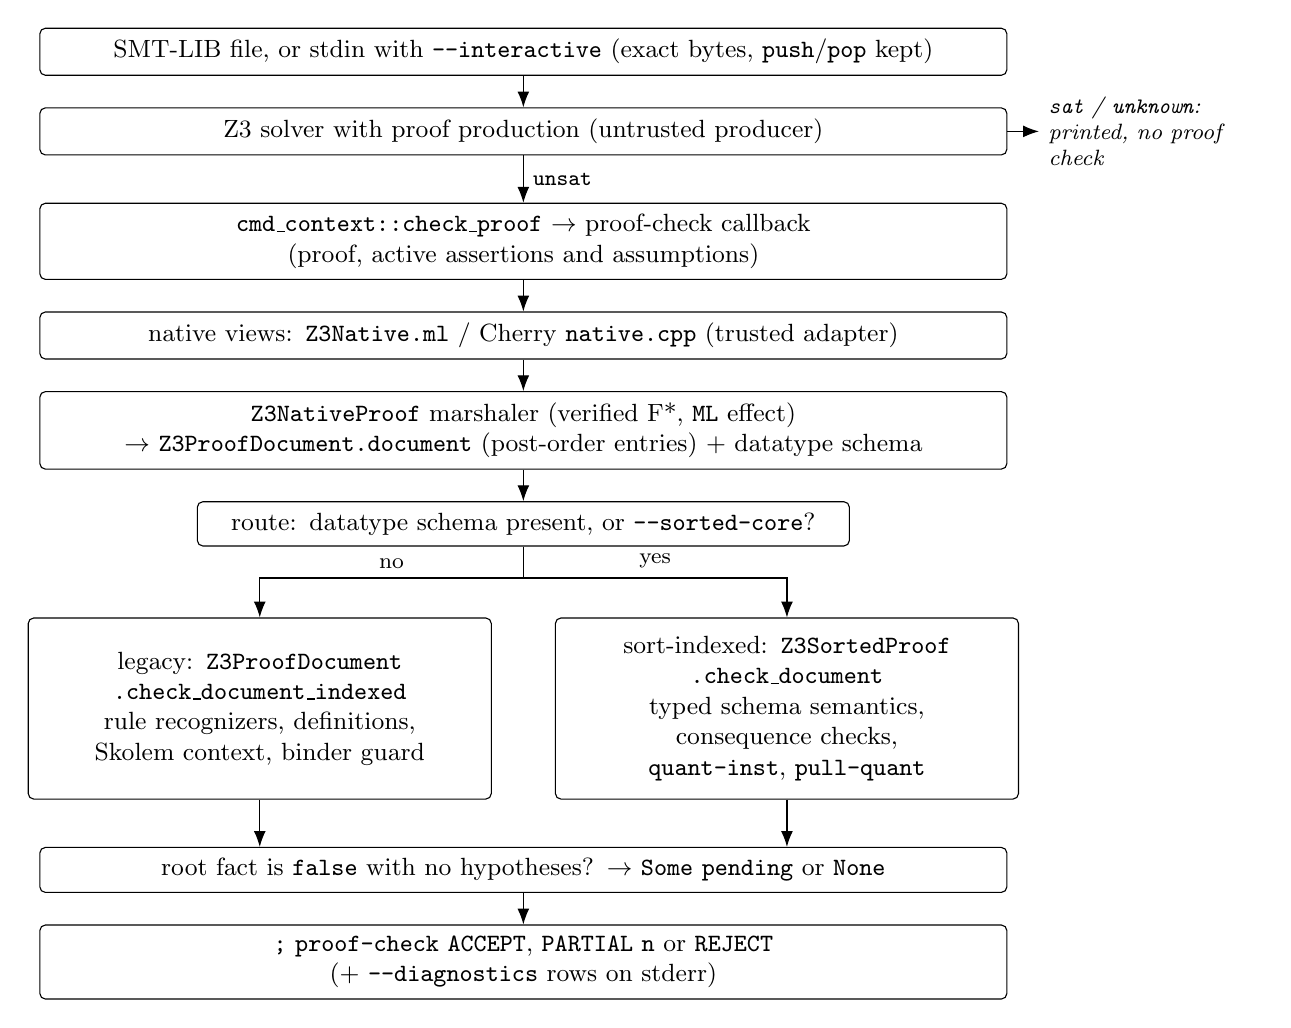
\begin{tikzpicture}[
  node distance=4mm,
  wide/.style={draw, rounded corners=2pt, align=center, font=\small, inner sep=4pt, text width=12cm},
  mid/.style={draw, rounded corners=2pt, align=center, font=\small, inner sep=4pt, text width=8cm},
  half/.style={draw, rounded corners=2pt, align=center, font=\small, inner sep=4pt, text width=5.6cm, minimum height=2.3cm},
  note/.style={font=\footnotesize\itshape, align=left, text width=2.6cm},
  lab/.style={font=\footnotesize},
  arr/.style={-{Latex[length=2mm]}}]
\node[wide] (in) {SMT-LIB file, or stdin with \texttt{-{}-interactive} (exact bytes, \texttt{push}/\texttt{pop} kept)};
\node[wide, below=of in] (z3) {Z3 solver with proof production (untrusted producer)};
\node[wide, below=6mm of z3] (cb) {\texttt{cmd\_context::check\_proof} $\rightarrow$ proof-check callback\\(proof, active assertions and assumptions)};
\node[wide, below=of cb] (view) {native views: \texttt{Z3Native.ml} / Cherry \texttt{native.cpp} (trusted adapter)};
\node[wide, below=of view] (marshal) {\texttt{Z3NativeProof} marshaler (verified F*, \texttt{ML} effect)\\$\rightarrow$ \texttt{Z3ProofDocument.document} (post-order entries) + datatype schema};
\node[mid, below=of marshal] (route) {route: datatype schema present, or \texttt{-{}-sorted-core}?};
\coordinate (split) at ([yshift=-9mm]route.south);
\node[half, anchor=north east] (legacy) at ([xshift=-4mm]split) {legacy: \texttt{Z3ProofDocument}\\\texttt{.check\_document\_indexed}\\rule recognizers, definitions,\\Skolem context, binder guard};
\node[half, anchor=north west] (sorted) at ([xshift=4mm]split) {sort-indexed: \texttt{Z3SortedProof}\\\texttt{.check\_document}\\typed schema semantics,\\consequence checks,\\\texttt{quant-inst}, \texttt{pull-quant}};
\coordinate (join) at (split |- legacy.south);
\node[wide, anchor=north] (root) at ([yshift=-6mm]join) {root fact is \texttt{false} with no hypotheses? $\rightarrow$ \texttt{Some pending} or \texttt{None}};
\node[wide, below=of root] (out) {\texttt{; proof-check ACCEPT}, \texttt{PARTIAL n} or \texttt{REJECT}\\(+ \texttt{-{}-diagnostics} rows on stderr)};
\draw[arr] (in) -- (z3);
\draw[arr] (z3) -- node[right, lab] {\texttt{unsat}} (cb);
\draw[arr] (z3.east) -- ++(4mm,0) node[note, right] {\texttt{sat} / \texttt{unknown}: printed, no proof check};
\draw[arr] (cb) -- (view);
\draw[arr] (view) -- (marshal);
\draw[arr] (marshal) -- (route);
\draw[arr] (route.south) -- ++(0,-4mm) -| node[pos=0.25, above, lab] {no} (legacy.north);
\draw[arr] (route.south) -- ++(0,-4mm) -| node[pos=0.25, above, lab] {yes} (sorted.north);
\draw[arr] (legacy.south) -- (legacy.south |- root.north);
\draw[arr] (sorted.south) -- (sorted.south |- root.north);
\draw[arr] (root) -- (out);
\end{tikzpicture}
\end{center}

\subsection{Input, solver and callback}\label{sec:31-input-solver-and-callback}

In file mode the OCaml driver parses the whole input with \texttt{parse\_\allowbreak{}smtlib2\_\allowbreak{}string}, asserts it, runs \texttt{solver\_\allowbreak{}check} and fetches the proof (\texttt{solve\_\allowbreak{}with\_\allowbreak{}clause\_\allowbreak{}proofs}, \href{https://github.com/Z3Prover/z3/blob/8fbb275aba0472e862e289c7af1331b3bd5d512c/fstar/ocaml_runtime/Z3Native.ml\#L543-L570}{ocaml\_\allowbreak{}runtime/\allowbreak{}Z3Native.\allowbreak{}ml}). The context is created with \texttt{proof=\allowbreak{}true} and the solver timeout. The Cherry driver does the same with the C++ API (\href{https://github.com/Z3Prover/z3/blob/8fbb275aba0472e862e289c7af1331b3bd5d512c/fstar/cherry_runtime/main.cpp\#L601-L647}{cherry\_\allowbreak{}runtime/\allowbreak{}main.\allowbreak{}cpp}).

\texttt{-{}\allowbreak{}-{}\allowbreak{}interactive} is the mode that preserves an incremental F* session. \texttt{read\_\allowbreak{}command} frames one complete command at a time from stdin, handling comments, quoted symbols and strings, without parsing SMT-LIB (\href{https://github.com/Z3Prover/z3/blob/8fbb275aba0472e862e289c7af1331b3bd5d512c/fstar/ocaml_runtime/Z3NativeMain.ml\#L208-L265}{ocaml\_\allowbreak{}runtime/\allowbreak{}Z3Native\allowbreak{}Main.\allowbreak{}ml}). Each command goes to \texttt{Z3\_\allowbreak{}eval\_\allowbreak{}smtlib2\_\allowbreak{}string} on one persistent context (\texttt{interactive}, \href{https://github.com/Z3Prover/z3/blob/8fbb275aba0472e862e289c7af1331b3bd5d512c/fstar/ocaml_runtime/Z3NativeMain.ml\#L267-L321}{ocaml\_\allowbreak{}runtime/\allowbreak{}Z3Native\allowbreak{}Main.\allowbreak{}ml}; Cherry \href{https://github.com/Z3Prover/z3/blob/8fbb275aba0472e862e289c7af1331b3bd5d512c/fstar/cherry_runtime/main.cpp\#L363-L542}{cherry\_\allowbreak{}runtime/\allowbreak{}main.\allowbreak{}cpp}). After \texttt{reset} the driver re-enables proof production, and a \texttt{set-{}\allowbreak{}option} that turns proofs off is undone and reported as an error. The process exit status is 2 if any command failed, else 1 if any proof was rejected, else 3 if any was partial, else 0.

The driver registers a callback with \texttt{Z3\_\allowbreak{}set\_\allowbreak{}proof\_\allowbreak{}check\_\allowbreak{}callback} (\href{https://github.com/Z3Prover/z3/blob/8fbb275aba0472e862e289c7af1331b3bd5d512c/src/api/z3_api.h\#L1735-L1761}{.\allowbreak{}.\allowbreak{}/\allowbreak{}src/\allowbreak{}api/\allowbreak{}z3\_\allowbreak{}api.\allowbreak{}h}). After an unsatisfiable \texttt{check-{}\allowbreak{}sat}, \texttt{check-{}\allowbreak{}sat-{}\allowbreak{}assuming} or \texttt{check-{}\allowbreak{}sat-{}\allowbreak{}using}, \texttt{cmd\_\allowbreak{}context:\allowbreak{}:\allowbreak{}check\_\allowbreak{}proof} collects the inputs and calls it (\href{https://github.com/Z3Prover/z3/blob/8fbb275aba0472e862e289c7af1331b3bd5d512c/src/cmd_context/cmd_context.cpp\#L2026-L2056}{.\allowbreak{}.\allowbreak{}/\allowbreak{}src/\allowbreak{}cmd\_\allowbreak{}context/\allowbreak{}cmd\_\allowbreak{}context.\allowbreak{}cpp}). The inputs are the tracked assertions of the current scope, with a named assertion passed as \texttt{name =\allowbreak{}> assertion} plus \texttt{name}, followed by the check's assumptions. The callback's report is printed as \texttt{; proof-{}\allowbreak{}check .\allowbreak{}.\allowbreak{}.\allowbreak{}} and \texttt{; proof-{}\allowbreak{}stats .\allowbreak{}.\allowbreak{}.\allowbreak{}} comment lines. Z3 does not interpret the report and does not change the \texttt{unsat} answer.

\subsection{Native views and marshaling}\label{sec:32-native-views-and-marshaling}

The foreign adapter is trusted code. \href{https://github.com/Z3Prover/z3/blob/8fbb275aba0472e862e289c7af1331b3bd5d512c/fstar/Z3Native.fsti}{Z3Native.\allowbreak{}fsti} declares abstract handles and view functions. The OCaml implementation \texttt{view\_\allowbreak{}proof} (\href{https://github.com/Z3Prover/z3/blob/8fbb275aba0472e862e289c7af1331b3bd5d512c/fstar/ocaml_runtime/Z3Native.ml\#L404-L501}{ocaml\_\allowbreak{}runtime/\allowbreak{}Z3Native.\allowbreak{}ml}) reads the rule name, the proof-sorted arguments as premises and the last argument as conclusion. It also reads arithmetic hints: Farkas and LP coefficients become candidate weights (L426-L453), the producer's \texttt{arith assumed <origin>} marker is recorded (L454-L457), and \texttt{th-{}\allowbreak{}lemma} nodes with an LP hint but no coefficients are renamed \texttt{arith/\allowbreak{}<hint>}, with \texttt{lp-{}\allowbreak{}context} renamed \texttt{def-{}\allowbreak{}axiom} (L458-L462). The Cherry adapter (\href{https://github.com/Z3Prover/z3/blob/8fbb275aba0472e862e289c7af1331b3bd5d512c/fstar/cherry_runtime/native.cpp\#L603-L631}{cherry\_\allowbreak{}runtime/\allowbreak{}native.\allowbreak{}cpp}) applies the same renaming. The corpus families \texttt{arith/\allowbreak{}lp-{}\allowbreak{}monomial-{}\allowbreak{}interval} and \texttt{arith/\allowbreak{}lp-{}\allowbreak{}monomial-{}\allowbreak{}substitute} in Appendix A get their names here; no F* source mentions them.

The marshaler \href{https://github.com/Z3Prover/z3/blob/8fbb275aba0472e862e289c7af1331b3bd5d512c/fstar/Z3NativeProof.fst}{Z3Native\allowbreak{}Proof.\allowbreak{}fst} is verified F* in the \texttt{ML} effect. It walks the native DAG with explicit worklists (\texttt{marshal\_\allowbreak{}expression\_\allowbreak{}jobs}, L169; \texttt{marshal\_\allowbreak{}proof\_\allowbreak{}jobs}, L423), caches expressions and proofs by native AST id, and emits entries in post-order so that premises are indices of earlier entries. \texttt{native\_\allowbreak{}rule} (L227-L244) maps the view to a rule: an \texttt{assumed} origin becomes \texttt{Unverified "assumed:\allowbreak{}<origin>"}, Farkas weights are accepted only on \texttt{th-{}\allowbreak{}lemma}, and a commutativity step is re-checked before it is labelled as one. \texttt{quant-{}\allowbreak{}intro}, \texttt{nnf-{}\allowbreak{}pos} and \texttt{nnf-{}\allowbreak{}neg} become \texttt{QuantifierIntrod\allowbreak{}uction} with a hidden binder certificate and an empty premise list (L287-L300, L477-L479). \texttt{quant-{}\allowbreak{}inst} keeps its instantiation terms, and \texttt{arith/\allowbreak{}lp-{}\allowbreak{}gomory} is rebuilt from the LP context certificate or left \texttt{Unverified} (L479-L495). \texttt{marshal\_\allowbreak{}with\_\allowbreak{}datatypes} returns the document together with the native datatype schema (L534).

The document type is \href{https://github.com/Z3Prover/z3/blob/8fbb275aba0472e862e289c7af1331b3bd5d512c/fstar/Z3ProofDocument.fst\#L16-L29}{Z3Proof\allowbreak{}Document.\allowbreak{}fst}: declarations, expressions, assertions, entries \texttt{\{rule; formula; premise\_\allowbreak{}ids\}} and a root index. Judgments are \texttt{Holds e}, \texttt{Equal a b} and \texttt{Observational a b}; a checked fact is a conclusion plus the open hypotheses it depends on (\href{https://github.com/Z3Prover/z3/blob/8fbb275aba0472e862e289c7af1331b3bd5d512c/fstar/Z3UnifiedProof.fst\#L1015-L1024}{Z3Unified\allowbreak{}Proof.\allowbreak{}fst}).

\subsection{Route choice}\label{sec:33-route-choice}

Both drivers pick a route per proof. If the marshaled schema has datatype cases, or \texttt{-{}\allowbreak{}-{}\allowbreak{}sorted-{}\allowbreak{}core} was given, the document goes to \texttt{Z3SortedProof.\allowbreak{}check\_\allowbreak{}document}. Otherwise it goes to the legacy \texttt{Z3ProofDocument.\allowbreak{}check\_\allowbreak{}document\_\allowbreak{}indexed} (\href{https://github.com/Z3Prover/z3/blob/8fbb275aba0472e862e289c7af1331b3bd5d512c/fstar/ocaml_runtime/Z3NativeMain.ml\#L156-L178}{ocaml\_\allowbreak{}runtime/\allowbreak{}Z3Native\allowbreak{}Main.\allowbreak{}ml}, \href{https://github.com/Z3Prover/z3/blob/8fbb275aba0472e862e289c7af1331b3bd5d512c/fstar/Z3Cherry.fst\#L54-L65}{Z3Cherry.\allowbreak{}fst}, \href{https://github.com/Z3Prover/z3/blob/8fbb275aba0472e862e289c7af1331b3bd5d512c/fstar/cherry_runtime/main.cpp\#L300-L301}{cherry\_\allowbreak{}runtime/\allowbreak{}main.\allowbreak{}cpp}). \texttt{-{}\allowbreak{}-{}\allowbreak{}stats} reports the route as \texttt{semantics=\allowbreak{}legacy}, \texttt{sorted-{}\allowbreak{}core} or \texttt{sorted-{}\allowbreak{}datatype}. There is no option that sends a datatype document to the legacy route, and the sort-indexed route has no legacy fallback (\href{https://github.com/Z3Prover/z3/blob/8fbb275aba0472e862e289c7af1331b3bd5d512c/fstar/PROOF_CHECKING.md\#L144-L150}{PROOF\_\allowbreak{}CHECKING.\allowbreak{}md}).

F* encodes its terms with SMT-LIB datatypes, so F* queries take the sort-indexed route. In the corpus run of Appendix A every checked query on both backends reported \texttt{semantics=\allowbreak{}sorted-{}\allowbreak{}datatype}.

\subsection{The legacy document checker}\label{sec:34-the-legacy-document-checker}

\href{https://github.com/Z3Prover/z3/blob/8fbb275aba0472e862e289c7af1331b3bd5d512c/fstar/Z3ProofDocument.fst}{Z3Proof\allowbreak{}Document.\allowbreak{}fst} prepares and checks one entry at a time in post-order. It filters declarations (\texttt{logical\_\allowbreak{}decls}), validates scopes for documents with binders, and collects definitions from \texttt{intro-{}\allowbreak{}def} and \texttt{def-{}\allowbreak{}axiom} entries (\texttt{collect\_\allowbreak{}definitions}, L53-L68). It expands fresh-bit reconstructions only when every input is within a 65,536-node budget (\texttt{document\_\allowbreak{}definitions}, L93-L108). Skolem definitions are collected and ordered. Each entry is prepared (definition expansion, judgment classification) and checked by \texttt{check\_\allowbreak{}node\_\allowbreak{}with\_\allowbreak{}membership} (\href{https://github.com/Z3Prover/z3/blob/8fbb275aba0472e862e289c7af1331b3bd5d512c/fstar/Z3UnifiedProof.fst\#L1084-L1130}{Z3Unified\allowbreak{}Proof.\allowbreak{}fst}), with premises looked up only among earlier ids in an id table.

\texttt{check\_\allowbreak{}node\_\allowbreak{}with\_\allowbreak{}membership} is where the rule kinds are dispatched. An \texttt{asserted} node must be an input. \texttt{hypothesis} introduces an open hypothesis, and \texttt{lemma} discharges it from a premise \texttt{false}. \texttt{def-{}\allowbreak{}axiom}, rewrite-like rules, \texttt{sk}, binder introductions and \texttt{quant-{}\allowbreak{}inst} must be premise-free and contribute 0 or 1 pending obligation depending on their recognizer. Theory lemmas, Farkas, Gomory and PAC certificates go through \texttt{checked\_\allowbreak{}theory\_\allowbreak{}lemma} (L1069-L1082). Core rules (\texttt{refl}, \texttt{symm}, \texttt{trans}, \texttt{monotonicity}, \texttt{mp}, \texttt{unit-{}\allowbreak{}resolution} and similar) must check or the node is rejected.

\texttt{finish\_\allowbreak{}document} and \texttt{finish\_\allowbreak{}table} require the root to be \texttt{Holds false} with no hypotheses and the defined symbols to be fresh in the inputs (\texttt{D.\allowbreak{}check\_\allowbreak{}fresh\_\allowbreak{}inputs}), and then return the summed pending count (\href{https://github.com/Z3Prover/z3/blob/8fbb275aba0472e862e289c7af1331b3bd5d512c/fstar/Z3ProofDocument.fst\#L520-L532}{Z3Proof\allowbreak{}Document.\allowbreak{}fst}).

\subsection{The sort-indexed document checker}\label{sec:35-the-sort-indexed-document-checker}

\href{https://github.com/Z3Prover/z3/blob/8fbb275aba0472e862e289c7af1331b3bd5d512c/fstar/Z3SortedProof.fst}{Z3Sorted\allowbreak{}Proof.\allowbreak{}fst} checks a document against a validated datatype schema with typed semantics. \texttt{check\_\allowbreak{}document} (L1070-L1079) rejects an invalid schema or ill-typed assertions, checks the entries, and applies the same root test as the legacy route.

The per-node function \texttt{check\_\allowbreak{}node\_\allowbreak{}cached} (L954-L979) reads less of a node than the legacy route does. It distinguishes five rule shapes. \texttt{asserted} must be premise-free and an input; \texttt{hypothesis} opens a hypothesis; \texttt{lemma} with a premise \texttt{false} discharges hypotheses; \texttt{quant-{}\allowbreak{}inst} is checked by \texttt{Z3SortedQuantifi\allowbreak{}er.\allowbreak{}check}; \texttt{pull-{}\allowbreak{}quant} by \texttt{check\_\allowbreak{}flatten}. Every other node is checked the same way, whatever its rule: the conclusion must follow from the premise conclusions by \texttt{consequence} (L734-L736: direct consequence and constructor-premise propagation with fuel 8) or by \texttt{DT.\allowbreak{}consequence} in \href{https://github.com/Z3Prover/z3/blob/8fbb275aba0472e862e289c7af1331b3bd5d512c/fstar/Z3SortedDatatype.fst}{Z3Sorted\allowbreak{}Datatype.\allowbreak{}fst}. If neither decides it, the node is kept with one pending obligation. \texttt{prepare\_\allowbreak{}entry\_\allowbreak{}from} (L1040-L1046) does no definition expansion.

So Farkas weights, Gomory and PAC certificates, binder certificates and Skolem definitions are not consulted on this route. A binder introduction arrives with no premises, because its premise is inside the certificate, and must be decided as a premise-free consequence. Draft PR \#11498 proves this reading property as a lemma (\href{https://github.com/Z3Prover/z3/blob/497dc106537fadc7633f78d9c91ac4dbfd7baf4b/fstar/Z3SortedRootDocument.fst\#L181-L247}{pinned Z3SortedRootDocument.fst\#L181-L247}). It follows that a rule name in the sort-indexed diagnostics names a node the sort-indexed procedure did not decide. It is not evidence that the legacy recognizer of that rule failed, because that recognizer did not run.

\subsection{Verdicts and diagnostics}\label{sec:36-verdicts-and-diagnostics}

\texttt{Some 0} prints \texttt{ACCEPT}, \texttt{Some n} prints \texttt{PARTIAL n} and \texttt{None} prints \texttt{REJECT} (\texttt{result\_\allowbreak{}text}, \href{https://github.com/Z3Prover/z3/blob/8fbb275aba0472e862e289c7af1331b3bd5d512c/fstar/ocaml_runtime/Z3NativeMain.ml\#L201-L204}{ocaml\_\allowbreak{}runtime/\allowbreak{}Z3Native\allowbreak{}Main.\allowbreak{}ml}; \href{https://github.com/Z3Prover/z3/blob/8fbb275aba0472e862e289c7af1331b3bd5d512c/fstar/cherry_runtime/main.cpp\#L357-L358}{cherry\_\allowbreak{}runtime/\allowbreak{}main.\allowbreak{}cpp}). In file mode the exit codes are 0 \texttt{ACCEPT}, 1 \texttt{REJECT}, 2 error, 3 \texttt{PARTIAL}, 4 \texttt{SAT} and 5 \texttt{UNKNOWN} (\href{https://github.com/Z3Prover/z3/blob/8fbb275aba0472e862e289c7af1331b3bd5d512c/fstar/OCAML_CHECKER_REPORT.md\#L2444-L2451}{OCAML\_\allowbreak{}CHECKER\_\allowbreak{}REPORT.\allowbreak{}md}).

\texttt{-{}\allowbreak{}-{}\allowbreak{}diagnostics} runs a diagnosing twin of the checker instead of the plain one and takes the verdict from it. F* proves that the twin's result equals the plain checker's (\texttt{Z3ProofDocument.\allowbreak{}fst} L585-L865, \texttt{Z3SortedProof.\allowbreak{}fst} L1180-L1273). The driver then prints \texttt{diagnostic checked pending=\allowbreak{}N families=\allowbreak{}K} and one row per group, \texttt{obligation <rule> <count> <first-{}\allowbreak{}node> <fingerprint>} (\href{https://github.com/Z3Prover/z3/blob/8fbb275aba0472e862e289c7af1331b3bd5d512c/fstar/ocaml_runtime/Z3NativeMain.ml\#L126-L154}{ocaml\_\allowbreak{}runtime/\allowbreak{}Z3Native\allowbreak{}Main.\allowbreak{}ml}; \href{https://github.com/Z3Prover/z3/blob/8fbb275aba0472e862e289c7af1331b3bd5d512c/fstar/cherry_runtime/main.cpp\#L234-L280}{cherry\_\allowbreak{}runtime/\allowbreak{}main.\allowbreak{}cpp}). The rule name comes from \texttt{diagnostic\_\allowbreak{}rule} (L7-L45). \texttt{th-{}\allowbreak{}lemma} covers both unverified theory lemmas and finite-field PAC steps, and the three binder rules report the binder certificate's root name. The fingerprint is lossy on purpose. It stops at depth 5 or 96 nodes and prints at most 8 arguments per application. Base sorts other than \texttt{Bool}, \texttt{Int} and \texttt{Real} (bit-vector, datatype and uninterpreted sorts) become \texttt{U}, while array sorts keep their index and element sorts to depth 2. Uninterpreted names are aliased to \texttt{u0}, \texttt{u1} and so on, rational numerals longer than 64 characters become \texttt{large-{}\allowbreak{}numeral}, and bit-vector values and binder sorts are dropped (L65-L121). It groups obligations; it is not a readable statement of the condition.

\section{Theory coverage}\label{sec:4-theory-coverage}

The table lists what the legacy route decides, under which guard, and what semantic assumption the decision rests on. "\texttt{model\_\allowbreak{}sound}" is the legacy global contract (\href{https://github.com/Z3Prover/z3/blob/8fbb275aba0472e862e289c7af1331b3bd5d512c/fstar/Z3UnifiedProof.fst\#L1164-L1175}{Z3Unified\allowbreak{}Proof.\allowbreak{}fst}), which is uninhabited (\hyperref[sec:51-the-legacy-global-contract-is-uninhabited]{section 5.1}). A family whose backing is \texttt{model\_\allowbreak{}sound} has a decision procedure and a node theorem whose assumption is uninhabited, so the theorem does not provide the intended soundness assurance.

{\footnotesize
\begin{longtable}{>{\raggedright\arraybackslash}p{\dimexpr 0.249\linewidth-2\tabcolsep\relax}>{\raggedright\arraybackslash}p{\dimexpr 0.249\linewidth-2\tabcolsep\relax}>{\raggedright\arraybackslash}p{\dimexpr 0.249\linewidth-2\tabcolsep\relax}>{\raggedright\arraybackslash}p{\dimexpr 0.249\linewidth-2\tabcolsep\relax}}
\toprule
\textbf{Family} & \textbf{Decision code} & \textbf{Fragment and guards} & \textbf{Semantic backing on master} \\
\midrule
\endfirsthead
\toprule
\textbf{Family} & \textbf{Decision code} & \textbf{Fragment and guards} & \textbf{Semantic backing on master} \\
\midrule
\endhead
\bottomrule
\endlastfoot
Boolean core and EUF (\texttt{refl}, \texttt{symm}, \texttt{trans}, \texttt{monotonicity}, \texttt{mp}, \texttt{unit-{}\allowbreak{}resolution}, \texttt{and-{}\allowbreak{}elim}, \texttt{not-{}\allowbreak{}or-{}\allowbreak{}elim}, \texttt{iff-{}\allowbreak{}true}, \texttt{iff-{}\allowbreak{}false}, \texttt{iff\textasciitilde{}}) & \texttt{relational\_\allowbreak{}step}, \texttt{logical\_\allowbreak{}step} (\href{https://github.com/Z3Prover/z3/blob/8fbb275aba0472e862e289c7af1331b3bd5d512c/fstar/Z3UnifiedProof.fst\#L272-L368}{Z3Unified\allowbreak{}Proof.\allowbreak{}fst}) & canonical connectives only & inhabited typed core model, per-node theorem \texttt{lemma\_\allowbreak{}core\_\allowbreak{}check\_\allowbreak{}node\_\allowbreak{}sound} (\href{https://github.com/Z3Prover/z3/blob/8fbb275aba0472e862e289c7af1331b3bd5d512c/fstar/Z3CoreKernel.fst\#L482-L526}{Z3Core\allowbreak{}Kernel.\allowbreak{}fst}) \\
Bounded bit-vector evaluation & \texttt{Z3BvExhaustive.\allowbreak{}valid} (\href{https://github.com/Z3Prover/z3/blob/8fbb275aba0472e862e289c7af1331b3bd5d512c/fstar/Z3BvExhaustive.fst\#L298-L308}{Z3Bv\allowbreak{}Exhaustive.\allowbreak{}fst}) & premise-free \texttt{th-{}\allowbreak{}lemma} and \texttt{rewrite}, closed ground terms, at most 512 nodes and 12 leaf bits (L64-L66) & core model through \texttt{lemma\_\allowbreak{}bv\_\allowbreak{}theory\_\allowbreak{}lemma} (\href{https://github.com/Z3Prover/z3/blob/8fbb275aba0472e862e289c7af1331b3bd5d512c/fstar/Z3CoreKernel.fst\#L458-L468}{Z3Core\allowbreak{}Kernel.\allowbreak{}fst}) \\
Other BV rewrites (\texttt{Z3BvAddNormalize\allowbreak{}}, \texttt{Z3BvExtract}, \texttt{Z3BvFresh}) & recognizers in \texttt{relational\_\allowbreak{}step} & per-recognizer bounds & \texttt{model\_\allowbreak{}sound} \\
Quantifier instantiation & \texttt{Z3QuantifierInst\allowbreak{}antiation.\allowbreak{}check} (\href{https://github.com/Z3Prover/z3/blob/8fbb275aba0472e862e289c7af1331b3bd5d512c/fstar/Z3QuantifierInstantiation.fst\#L15-L24}{Z3Quantifier\allowbreak{}Instantiation.\allowbreak{}fst}) & closed arguments whose sorts match the binders, capture-avoiding substitution & typed quantifier model, \texttt{lemma\_\allowbreak{}typed\_\allowbreak{}check\_\allowbreak{}node\_\allowbreak{}sound} (\href{https://github.com/Z3Prover/z3/blob/8fbb275aba0472e862e289c7af1331b3bd5d512c/fstar/Z3QuantifierKernel.fst\#L181-L192}{Z3Quantifier\allowbreak{}Kernel.\allowbreak{}fst}) \\
Binder introduction (\texttt{quant-{}\allowbreak{}intro}, \texttt{nnf-{}\allowbreak{}pos}, \texttt{nnf-{}\allowbreak{}neg}) & \texttt{binder\_\allowbreak{}step} (\href{https://github.com/Z3Prover/z3/blob/8fbb275aba0472e862e289c7af1331b3bd5d512c/fstar/Z3UnifiedProof.fst\#L478-L493}{Z3Unified\allowbreak{}Proof.\allowbreak{}fst}), scope guard \texttt{binder\_\allowbreak{}scoped} (L987-L999) & typed theorem only for closed inputs, core rules and exact forall/exists introductions (\href{https://github.com/Z3Prover/z3/blob/8fbb275aba0472e862e289c7af1331b3bd5d512c/fstar/Z3BinderKernel.fst\#L543-L554}{Z3Binder\allowbreak{}Kernel.\allowbreak{}fst}); guard limits in \href{https://github.com/Z3Prover/z3/blob/8fbb275aba0472e862e289c7af1331b3bd5d512c/fstar/Z3UnifiedProof.fst\#L611-L619}{Z3Unified\allowbreak{}Proof.\allowbreak{}fst} & restricted fragment: typed quantifier model; the rest: \texttt{model\_\allowbreak{}sound} \\
Skolemization (\texttt{sk}) & \texttt{Z3Skolemization.\allowbreak{}check} (\href{https://github.com/Z3Prover/z3/blob/8fbb275aba0472e862e289c7af1331b3bd5d512c/fstar/Z3Skolemization.fst\#L231}{Z3Skolemization.\allowbreak{}fst}) & one Hilbert-choice tuple per block, acyclic, fresh in the inputs & \texttt{model\_\allowbreak{}sound} plus the Skolem context model \\
Boolean normalization, \texttt{def-{}\allowbreak{}axiom}, \texttt{intro-{}\allowbreak{}def} & \texttt{D.\allowbreak{}tautology 128} (\href{https://github.com/Z3Prover/z3/blob/8fbb275aba0472e862e289c7af1331b3bd5d512c/fstar/Z3Definitions.fst\#L476-L490}{Z3Definitions.\allowbreak{}fst}), Boolean search & fuel and size budgets & \texttt{model\_\allowbreak{}sound} \\
\texttt{rewrite} & disjunction of recognizers (\href{https://github.com/Z3Prover/z3/blob/8fbb275aba0472e862e289c7af1331b3bd5d512c/fstar/Z3UnifiedProof.fst\#L283-L300}{Z3Unified\allowbreak{}Proof.\allowbreak{}fst}): identity, flattening, \texttt{distinct}, arrays, arithmetic, factoring, BV extract, quantifier reduction, lambdas, conditionals, integers, division, vacuity, theory normalization, Boolean search & per-recognizer budgets & \texttt{model\_\allowbreak{}sound}, except the bounded BV case \\
Linear arithmetic, Farkas & \texttt{LA.\allowbreak{}check} (\href{https://github.com/Z3Prover/z3/blob/8fbb275aba0472e862e289c7af1331b3bd5d512c/fstar/Z3LinearArithmeticAst.fst\#L176-L180}{Z3Linear\allowbreak{}Arithmetic\allowbreak{}Ast.\allowbreak{}fst}) with producer weights as candidates & Int and Real linear; integer strict-bound rounding not applied to Real & \texttt{model\_\allowbreak{}sound} (numeric model) \\
LP replay, Gomory and integer cuts & \href{https://github.com/Z3Prover/z3/blob/8fbb275aba0472e862e289c7af1331b3bd5d512c/fstar/Z3LpReplay.fst\#L44-L86}{Z3Lp\allowbreak{}Replay.\allowbreak{}fst}, \href{https://github.com/Z3Prover/z3/blob/8fbb275aba0472e862e289c7af1331b3bd5d512c/fstar/Z3LpGomory.fst\#L43}{Z3Lp\allowbreak{}Gomory.\allowbreak{}fst}, \href{https://github.com/Z3Prover/z3/blob/8fbb275aba0472e862e289c7af1331b3bd5d512c/fstar/Z3LpIntegerCut.fst\#L49}{Z3Lp\allowbreak{}Integer\allowbreak{}Cut.\allowbreak{}fst} & replay at most 32 literals, 16 rounds, 128 rows (\href{https://github.com/Z3Prover/z3/blob/8fbb275aba0472e862e289c7af1331b3bd5d512c/fstar/PROOF_CHECKING.md\#L196-L204}{PROOF\_\allowbreak{}CHECKING.\allowbreak{}md}); cuts at most 32 premises, 128 rows, 8 cuts, 64 terms, 4,096 work units, magnitude 2\textasciicircum{}128 (\href{https://github.com/Z3Prover/z3/blob/8fbb275aba0472e862e289c7af1331b3bd5d512c/fstar/Z3LpIntegerCut.fst\#L81-L86}{Z3Lp\allowbreak{}Integer\allowbreak{}Cut.\allowbreak{}fst}) & \texttt{model\_\allowbreak{}sound} \\
\texttt{arith/\allowbreak{}lp-{}\allowbreak{}monomial-{}\allowbreak{}*}, \texttt{assumed:\allowbreak{}nlsat} & none on the legacy route; \texttt{checked\_\allowbreak{}theory\_\allowbreak{}lemma} accepts only \texttt{arith/\allowbreak{}lp-{}\allowbreak{}integer-{}\allowbreak{}tighten} among \texttt{Unverified} tags (\href{https://github.com/Z3Prover/z3/blob/8fbb275aba0472e862e289c7af1331b3bd5d512c/fstar/Z3UnifiedProof.fst\#L1079-L1080}{Z3Unified\allowbreak{}Proof.\allowbreak{}fst}) & always pending there & none \\
Arrays & \texttt{Z3ArrayLemma.\allowbreak{}array\_\allowbreak{}lemma} (\href{https://github.com/Z3Prover/z3/blob/8fbb275aba0472e862e289c7af1331b3bd5d512c/fstar/Z3ArrayLemma.fst\#L89}{Z3Array\allowbreak{}Lemma.\allowbreak{}fst}), \texttt{Z3ArrayRewrite}, \texttt{Z3ArrayEquality} & one-dimensional scalar index and element sorts & \texttt{model\_\allowbreak{}sound}, whose array clauses are inconsistent for Real elements (section 5.1) \\
Datatypes & sort-indexed route only: \href{https://github.com/Z3Prover/z3/blob/8fbb275aba0472e862e289c7af1331b3bd5d512c/fstar/Z3SortedDatatype.fst}{Z3Sorted\allowbreak{}Datatype.\allowbreak{}fst}, schema validity \href{https://github.com/Z3Prover/z3/blob/8fbb275aba0472e862e289c7af1331b3bd5d512c/fstar/Z3DatatypeSignature.fst\#L82-L87}{Z3Datatype\allowbreak{}Signature.\allowbreak{}fst} & arrays containing datatypes are rejected as constructor fields by \texttt{supported\_\allowbreak{}fields} (\href{https://github.com/Z3Prover/z3/blob/8fbb275aba0472e862e289c7af1331b3bd5d512c/fstar/Z3DatatypeSignature.fst\#L55-L59}{Z3Datatype\allowbreak{}Signature.\allowbreak{}fst}); sequences of datatypes are rejected earlier by the native adapter (\href{https://github.com/Z3Prover/z3/blob/8fbb275aba0472e862e289c7af1331b3bd5d512c/fstar/ocaml_runtime/Z3Native.ml\#L223-L227}{ocaml\_\allowbreak{}runtime/\allowbreak{}Z3Native.\allowbreak{}ml}, an \texttt{ERROR}) & typed sort-indexed semantics; document theorem conditional (section 5.3) \\
Finite fields & \texttt{FF.\allowbreak{}exhaustive\_\allowbreak{}clause}, \texttt{FF.\allowbreak{}equivalent} (\href{https://github.com/Z3Prover/z3/blob/8fbb275aba0472e862e289c7af1331b3bd5d512c/fstar/Z3FiniteFieldLemma.fst\#L964}{Z3Finite\allowbreak{}Field\allowbreak{}Lemma.\allowbreak{}fst}), PAC replay (\href{https://github.com/Z3Prover/z3/blob/8fbb275aba0472e862e289c7af1331b3bd5d512c/fstar/Z3FiniteFieldPac.fst\#L345}{Z3Finite\allowbreak{}Field\allowbreak{}Pac.\allowbreak{}fst}) & single modulus, bounded assignments; PAC steps needing a disequality inverse witness stay pending (\href{https://github.com/Z3Prover/z3/blob/8fbb275aba0472e862e289c7af1331b3bd5d512c/fstar/PROOF_CHECKING.md\#L77}{PROOF\_\allowbreak{}CHECKING.\allowbreak{}md}) & \texttt{model\_\allowbreak{}sound} (normalization model) \\
Floating point, strings, sequences, regular expressions & no native kernel branch; operators arrive as opaque declarations, except binary sequence concatenation, which is tagged (\texttt{OP\_\allowbreak{}SEQ\_\allowbreak{}CONCAT}, \href{https://github.com/Z3Prover/z3/blob/8fbb275aba0472e862e289c7af1331b3bd5d512c/fstar/ocaml_runtime/Z3Native.ml\#L129}{ocaml\_\allowbreak{}runtime/\allowbreak{}Z3Native.\allowbreak{}ml}) & congruence only & none \\*
\end{longtable}
}

On the sort-indexed route the table does not apply. That route decides Boolean and equality reasoning, datatype constructor, recognizer and accessor reasoning, quantifier instantiation and \texttt{pull-{}\allowbreak{}quant}, and integer operations through \href{https://github.com/Z3Prover/z3/blob/8fbb275aba0472e862e289c7af1331b3bd5d512c/fstar/Z3SortedInteger.fst}{Z3Sorted\allowbreak{}Integer.\allowbreak{}fst} and \href{https://github.com/Z3Prover/z3/blob/8fbb275aba0472e862e289c7af1331b3bd5d512c/fstar/Z3SortedArithmetic.fst}{Z3Sorted\allowbreak{}Arithmetic.\allowbreak{}fst}. Real arithmetic is abstract on that route, and no legacy theory recognizer runs on it.

\section{Formal assurance}\label{sec:5-formal-assurance}

\subsection{The legacy global contract is uninhabited}\label{sec:51-the-legacy-global-contract-is-uninhabited}

The legacy kernel theorem \texttt{lemma\_\allowbreak{}check\_\allowbreak{}node\_\allowbreak{}sound} (\href{https://github.com/Z3Prover/z3/blob/8fbb275aba0472e862e289c7af1331b3bd5d512c/fstar/Z3UnifiedProof.fst\#L1884-L1961}{Z3Unified\allowbreak{}Proof.\allowbreak{}fst}) assumes \texttt{model\_\allowbreak{}sound i} (\href{https://github.com/Z3Prover/z3/blob/8fbb275aba0472e862e289c7af1331b3bd5d512c/fstar/Z3UnifiedProof.fst\#L1164-L1175}{Z3Unified\allowbreak{}Proof.\allowbreak{}fst}). That predicate conjoins Boolean, arithmetic, array, quantifier, lambda, normalization and numeric contracts stated over all environments of an untyped value domain. Three of them are refuted outright in \href{https://github.com/Z3Prover/z3/blob/8fbb275aba0472e862e289c7af1331b3bd5d512c/fstar/Z3ScopedModelTests.fst}{Z3Scoped\allowbreak{}Model\allowbreak{}Tests.\allowbreak{}fst}, each lemma proving \texttt{False} from the contract:

\begin{itemize}\setlength{\itemsep}{1pt}\setlength{\parskip}{0pt}

\item \texttt{boolean\_\allowbreak{}model} asks every Bool-sorted term to evaluate to a Boolean under every environment. Under an environment that maps variable 0 to an integer, the Bool variable \texttt{Var 0} evaluates to that integer (\texttt{lemma\_\allowbreak{}legacy\_\allowbreak{}boolean\_\allowbreak{}contract\_\allowbreak{}impossible}, L11-L16).

\item \texttt{numeric\_\allowbreak{}model} asks the same of Int-sorted terms; a Bool-valued environment refutes it (\texttt{lemma\_\allowbreak{}legacy\_\allowbreak{}integer\_\allowbreak{}contract\_\allowbreak{}impossible}, L18-L23).

\item \texttt{array\_\allowbreak{}model} asks \texttt{select} arguments to be arrays; an array-sorted variable under a Bool-valued environment refutes it (\texttt{lemma\_\allowbreak{}legacy\_\allowbreak{}array\_\allowbreak{}contract\_\allowbreak{}impossible}, L25-L35).

\end{itemize}

Closed terms fail as well. In \href{https://github.com/Z3Prover/z3/blob/8fbb275aba0472e862e289c7af1331b3bd5d512c/fstar/Z3CoreModelTests.fst\#L462-L543}{Z3Core\allowbreak{}Model\allowbreak{}Tests.\allowbreak{}fst} the array-store, numeral and integer-coercion clause instances at \texttt{(\allowbreak{}store a 0 1/\allowbreak{}2)} with \texttt{a :\allowbreak{} (\allowbreak{}Array Int Real)} are jointly unsatisfiable (\texttt{o1\_\allowbreak{}clash}), while each pair of them is satisfiable (\texttt{drop\_\allowbreak{}s}, \texttt{drop\_\allowbreak{}n}, \texttt{drop\_\allowbreak{}i}). The untyped binder clause fails at an ill-typed value list: instantiated at \texttt{[true]}, it makes the valid closed formula \texttt{forall x:\allowbreak{}Int.\allowbreak{} x + 0 =\allowbreak{} x} false in every model of the quantifier, arithmetic and equality contracts (\texttt{o2\_\allowbreak{}unfaithful}, \href{https://github.com/Z3Prover/z3/blob/8fbb275aba0472e862e289c7af1331b3bd5d512c/fstar/Z3CoreModelTests.fst\#L545-L575}{Z3Core\allowbreak{}Model\allowbreak{}Tests.\allowbreak{}fst}).

F* accepts conditional statements from these assumptions, so \texttt{lemma\_\allowbreak{}check\_\allowbreak{}node\_\allowbreak{}sound} holds vacuously. The implication is vacuous: it does not provide the intended soundness assurance for any legacy \texttt{ACCEPT}. The legacy route also has no document-level soundness theorem. Every family in the table of \hyperref[sec:4-theory-coverage]{section 4} whose backing is \texttt{model\_\allowbreak{}sound} therefore has no non-vacuous formal guarantee today. This is the main open formal problem of the checker, and no merged or draft change replaces \texttt{model\_\allowbreak{}sound}.

\subsection{Inhabited guarantees on master}\label{sec:52-inhabited-guarantees-on-master}

\begin{itemize}\setlength{\itemsep}{1pt}\setlength{\parskip}{0pt}

\item \textbf{Typed core (\#11450).} \texttt{core\_\allowbreak{}model i dom} (\href{https://github.com/Z3Prover/z3/blob/8fbb275aba0472e862e289c7af1331b3bd5d512c/fstar/Z3CoreModel.fst\#L183-L186}{Z3Core\allowbreak{}Model.\allowbreak{}fst}) covers typing, canonical connectives, typed equality, integer \texttt{+} and \texttt{*}, and ground bit-vectors. \texttt{lemma\_\allowbreak{}core\_\allowbreak{}inhabited} (L318) proves a witness exists, and the classical ghost model \texttt{Z3GhostStandardM\allowbreak{}odel} is another witness (\texttt{lemma\_\allowbreak{}ghost\_\allowbreak{}inhabited}, \href{https://github.com/Z3Prover/z3/blob/8fbb275aba0472e862e289c7af1331b3bd5d512c/fstar/Z3GhostStandardModel.fst\#L479}{Z3Ghost\allowbreak{}Standard\allowbreak{}Model.\allowbreak{}fst}). \texttt{lemma\_\allowbreak{}core\_\allowbreak{}check\_\allowbreak{}node\_\allowbreak{}sound} (\href{https://github.com/Z3Prover/z3/blob/8fbb275aba0472e862e289c7af1331b3bd5d512c/fstar/Z3CoreKernel.fst\#L482-L526}{Z3Core\allowbreak{}Kernel.\allowbreak{}fst}) is a per-node theorem for the core rules and bounded BV.

\item \textbf{Typed quantifier instantiation (\#11450).} \texttt{quantifier\_\allowbreak{}model} (\href{https://github.com/Z3Prover/z3/blob/8fbb275aba0472e862e289c7af1331b3bd5d512c/fstar/Z3TypedQuantifier.fst\#L45-L53}{Z3Typed\allowbreak{}Quantifier.\allowbreak{}fst}) lets quantifiers range exactly over value lists typed by their binders. The ghost standard model realizes it (\texttt{lemma\_\allowbreak{}quantifier\_\allowbreak{}model}, \href{https://github.com/Z3Prover/z3/blob/8fbb275aba0472e862e289c7af1331b3bd5d512c/fstar/Z3GhostStandardModel.fst\#L486-L491}{Z3Ghost\allowbreak{}Standard\allowbreak{}Model.\allowbreak{}fst}), and \texttt{lemma\_\allowbreak{}typed\_\allowbreak{}check\_\allowbreak{}node\_\allowbreak{}sound} (\href{https://github.com/Z3Prover/z3/blob/8fbb275aba0472e862e289c7af1331b3bd5d512c/fstar/Z3QuantifierKernel.fst\#L181-L192}{Z3Quantifier\allowbreak{}Kernel.\allowbreak{}fst}) covers instantiation steps with no pending obligation.

\item \textbf{Restricted binder fragment (\#11493).} The scope guard \texttt{binder\_\allowbreak{}scoped} (\href{https://github.com/Z3Prover/z3/blob/8fbb275aba0472e862e289c7af1331b3bd5d512c/fstar/Z3UnifiedProof.fst\#L987-L999}{Z3Unified\allowbreak{}Proof.\allowbreak{}fst}) and the structural theorems of \href{https://github.com/Z3Prover/z3/blob/8fbb275aba0472e862e289c7af1331b3bd5d512c/fstar/Z3BinderScope.fst}{Z3Binder\allowbreak{}Scope.\allowbreak{}fst} support \texttt{lemma\_\allowbreak{}typed\_\allowbreak{}binder\_\allowbreak{}check\_\allowbreak{}node\_\allowbreak{}sound} (\href{https://github.com/Z3Prover/z3/blob/8fbb275aba0472e862e289c7af1331b3bd5d512c/fstar/Z3BinderKernel.fst\#L543-L554}{Z3Binder\allowbreak{}Kernel.\allowbreak{}fst}) for closed inputs, core rules and exact forall/exists introductions. \texttt{nnf} steps without sorts, \texttt{sk}, \texttt{rewrite}, \texttt{th-{}\allowbreak{}lemma} and \texttt{def-{}\allowbreak{}axiom} inside certificates are outside this fragment.

\end{itemize}

These are node-level theorems for fragments of the legacy route. A \texttt{Some} result of a node check does not by itself mean zero obligations, and no merged document theorem combines them into a statement about a native \texttt{ACCEPT}.

\subsection{The sort-indexed document theorem is conditional}\label{sec:53-the-sort-indexed-document-theorem-is-conditional}

\texttt{Z3SortedProof.\allowbreak{}lemma\_\allowbreak{}check\_\allowbreak{}document} (\href{https://github.com/Z3Prover/z3/blob/8fbb275aba0472e862e289c7af1331b3bd5d512c/fstar/Z3SortedProof.fst\#L1162-L1178}{Z3Sorted\allowbreak{}Proof.\allowbreak{}fst}) states that if \texttt{check\_\allowbreak{}document} returns \texttt{Some 0} then the assertions are not all true in the given typed interpretation. Its hypotheses include \texttt{Q.\allowbreak{}forall\_\allowbreak{}elimination\_\allowbreak{}model} when the document contains instantiation steps, and \texttt{Q.\allowbreak{}forall\_\allowbreak{}model} when it contains \texttt{pull-{}\allowbreak{}quant} steps (L1166-L1167); a document with neither needs no quantifier hypothesis. No lemma on master constructs an interpretation that satisfies those hypotheses, so for documents with instantiation or \texttt{pull-{}\allowbreak{}quant} steps the theorem is relative to an assumption that master's source does not construct. That is a statement about master's proofs, not a claim that the hypotheses are false or that the theorem is vacuous.

\subsection{Draft \#11498: an inhabited typed root (not merged)}\label{sec:54-draft-11498-an-inhabited-typed-root-not-merged}

\href{https://github.com/Z3Prover/z3/pull/11498}{PR \#11498} is open and in draft state, head \texttt{497dc106537fadc7\allowbreak{}633f78d9c91ac4db\allowbreak{}fd7baf4b}, base \texttt{8fbb275ab}. Nothing in this subsection is on master.

\begin{itemize}\setlength{\itemsep}{1pt}\setlength{\parskip}{0pt}

\item \texttt{Z3TypedRoot.\allowbreak{}fst} gives typed carriers: \texttt{bool}, \texttt{int}, \texttt{FStar.\allowbreak{}Real.\allowbreak{}real}, full ghost function spaces for arrays, an arbitrary nonempty model-chosen type for each other base sort, and checked constructor trees for datatypes (\href{https://github.com/Z3Prover/z3/blob/497dc106537fadc7633f78d9c91ac4dbfd7baf4b/fstar/Z3TypedRoot.fst\#L1-L60}{pinned Z3TypedRoot.fst\#L1-L60}). \texttt{root\_\allowbreak{}model} joins six laws, R1 quantifiers, R2 operators, R3 lambdas, R4 constructors, R5 recognizers and R6 accessors (\href{https://github.com/Z3Prover/z3/blob/497dc106537fadc7633f78d9c91ac4dbfd7baf4b/fstar/Z3TypedRoot.fst\#L693-L778}{pinned Z3TypedRoot.fst\#L693-L778}). \texttt{lemma\_\allowbreak{}standard\_\allowbreak{}root} and \texttt{lemma\_\allowbreak{}root\_\allowbreak{}inhabited} prove that a standard root model exists for every carrier family and every choice of free symbols (\href{https://github.com/Z3Prover/z3/blob/497dc106537fadc7633f78d9c91ac4dbfd7baf4b/fstar/Z3TypedRoot.fst\#L910-L930}{pinned Z3TypedRoot.fst\#L910-L930}).

\item \texttt{Z3SortedRootDocu\allowbreak{}ment.\allowbreak{}fst} derives the two quantifier hypotheses of section 5.3 from R1 and proves \texttt{lemma\_\allowbreak{}root\_\allowbreak{}check\_\allowbreak{}document}: if \texttt{check\_\allowbreak{}document} returns \texttt{Some 0}, the assertions are not all true in any root model (\href{https://github.com/Z3Prover/z3/blob/497dc106537fadc7633f78d9c91ac4dbfd7baf4b/fstar/Z3SortedRootDocument.fst\#L77-L176}{pinned Z3SortedRootDocument.fst\#L77-L176}).

\item \texttt{check\_\allowbreak{}root\_\allowbreak{}document} is a gate that reuses the unchanged sort-indexed decision and returns \texttt{RootCertified}, \texttt{RootUncovered}, \texttt{RootPending n} or \texttt{RootRejected}. \texttt{RootCertified} also requires a supported schema and covered, typed document terms. \texttt{lemma\_\allowbreak{}root\_\allowbreak{}certified} and \texttt{lemma\_\allowbreak{}standard\_\allowbreak{}certified} state the certified result for every root model and for the standard one (\href{https://github.com/Z3Prover/z3/blob/497dc106537fadc7633f78d9c91ac4dbfd7baf4b/fstar/Z3SortedRootDocument.fst\#L273-L300}{pinned Z3SortedRootDocument.fst\#L273-L300}, \href{https://github.com/Z3Prover/z3/blob/497dc106537fadc7633f78d9c91ac4dbfd7baf4b/fstar/Z3SortedRootDocument.fst\#L369-L393}{\#\allowbreak{}L369-L393}).

\item The gate is off the default route. The source comment says "No route calls it." At the pinned head, the Root modules are listed only under \texttt{tests} in \texttt{checker\_\allowbreak{}modules.\allowbreak{}json}, so they are verified only in builds with \texttt{-{}\allowbreak{}RunTests} and are never extracted (\href{https://github.com/Z3Prover/z3/blob/497dc106537fadc7633f78d9c91ac4dbfd7baf4b/fstar/tools/checker_modules.json\#L24-L32}{pinned checker\_modules.json\#L24-L32}), and the drivers still call \texttt{Z3SortedProof.\allowbreak{}check\_\allowbreak{}document}. A native sort-indexed \texttt{ACCEPT} is therefore not a \texttt{RootCertified} verdict, with or without this PR.

\end{itemize}

The draft theorem is relative. It quantifies over the class of root models, which is a metatheoretic choice: it does not prove that every SMT-LIB model of the input is a root model, and it trusts the native translation of assertions, schema and datatype metadata. The sort-indexed decision procedure does no Real, array, bit-vector, finite-field, sequence or floating-point reasoning. In the root model, Real arithmetic and datatype-free arrays are interpreted, while bit-vector, finite-field, sequence and floating-point operators are free choices. The legacy \texttt{model\_\allowbreak{}sound} is unchanged and still uninhabited, and the default route is unchanged.

The draft also moves semantic assertions out of the native test harness. With the typed datatype semantics made ghost, \texttt{concrete\_\allowbreak{}datatype\_\allowbreak{}model} in \texttt{tools/\allowbreak{}test\_\allowbreak{}native\_\allowbreak{}bridge.\allowbreak{}ml} can no longer run them, so the draft removes seven executable \texttt{require} checks and proves the same facts, with exact expected values and refuted wrong-value mutants, in a new F* test module on the same \texttt{Tree}/\texttt{Forest} fixture (\href{https://github.com/Z3Prover/z3/blob/497dc106537fadc7633f78d9c91ac4dbfd7baf4b/fstar/Z3DatatypeNativeModelTests.fst\#L1-L36}{pinned Z3DatatypeNativeModelTests.fst\#L1-L36}). On master these remain executable runtime checks.

\section{Extraction, runtime and build}\label{sec:6-extraction-runtime-and-build}

\textbf{Ghost semantics, total checking.} The interpretation fields and \texttt{eval} in \href{https://github.com/Z3Prover/z3/blob/8fbb275aba0472e862e289c7af1331b3bd5d512c/fstar/Z3AstTheory.fst\#L289-L325}{Z3Ast\allowbreak{}Theory.\allowbreak{}fst} are ghost (\texttt{GTot}), so models may decide classical propositions. Checking functions are \texttt{Tot} or \texttt{ML}, and F* rejects ghost results in executable code. Proofs that run an executable evaluator under a ghost valuation use ghost twins (\href{https://github.com/Z3Prover/z3/blob/8fbb275aba0472e862e289c7af1331b3bd5d512c/fstar/PROOF_CHECKING.md\#L55}{PROOF\_\allowbreak{}CHECKING.\allowbreak{}md}).

\textbf{Two backends from one source.} The OCaml backend extracts the verified modules with Custard (\texttt{-{}\allowbreak{}-{}\allowbreak{}codegen OCaml -{}\allowbreak{}-{}\allowbreak{}custard\_\allowbreak{}split}) and links them in dependency order. The Cherry backend generates C for the kernel and a C++ driver; it needs a Cherry-capable F* and GCC/G++ 15. Both executables link static Z3 and solve, marshal and check in one process; their options, incremental protocol, diagnostics and exit codes are the same (\href{https://github.com/Z3Prover/z3/blob/8fbb275aba0472e862e289c7af1331b3bd5d512c/fstar/README.md\#L56-L66}{README.\allowbreak{}md}). CI pins F* \texttt{v2026.\allowbreak{}10.\allowbreak{}25} for OCaml and \texttt{nightly-{}\allowbreak{}2026-{}\allowbreak{}10-{}\allowbreak{}30} for Cherry, OCaml 5.3.0 and GCC 15 (\href{https://github.com/Z3Prover/z3/blob/8fbb275aba0472e862e289c7af1331b3bd5d512c/.github/workflows/pulse-checker-build.yml\#L40-L91}{.\allowbreak{}.\allowbreak{}/\allowbreak{}.\allowbreak{}github/\allowbreak{}workflows/\allowbreak{}pulse-checker-build.\allowbreak{}yml}).

\textbf{\#11478 (merged).} This change bumped F*, inlined the option binds with \texttt{[@@custard\_\allowbreak{}inline]} (\href{https://github.com/Z3Prover/z3/blob/8fbb275aba0472e862e289c7af1331b3bd5d512c/fstar/Z3ProofIndex.fst\#L3-L10}{Z3Proof\allowbreak{}Index.\allowbreak{}fst}), made list helpers tail-recursive (\href{https://github.com/Z3Prover/z3/blob/8fbb275aba0472e862e289c7af1331b3bd5d512c/fstar/Z3List.fst}{Z3List.\allowbreak{}fst}), boxed the document and marshaler state records with \texttt{[@@cherry\_\allowbreak{}boxed]}, and replaced the Cherry proof-id caches with immutable arrays (\texttt{Z3IdTable-{}\allowbreak{}c.\allowbreak{}cherry.\allowbreak{}fst}). Its description reports (not reproduced here) that all 15 previously crashing CI inputs complete under the default 8 MB stack and under a 1 MB stack, without stack-size tweaks.

\textbf{\#11493 (merged).} The binder scope guard walks expressions and sorts with explicit worklists (\href{https://github.com/Z3Prover/z3/blob/8fbb275aba0472e862e289c7af1331b3bd5d512c/fstar/Z3UnifiedProof.fst\#L573-L590}{Z3Unified\allowbreak{}Proof.\allowbreak{}fst}). Its own comment limits the claim: "This is not a stack bound for the whole checker." It also added a trusted runtime binding for \texttt{list\_\allowbreak{}of\_\allowbreak{}string} (\href{https://github.com/Z3Prover/z3/blob/8fbb275aba0472e862e289c7af1331b3bd5d512c/fstar/ocaml_runtime/fStar_String.ml}{ocaml\_\allowbreak{}runtime/\allowbreak{}f\allowbreak{}Star\_\allowbreak{}String.\allowbreak{}ml}).

\textbf{Trusted base.} Beyond Z3 itself, the trusted code is the F* extraction and the two runtimes: the files of \texttt{ocaml\_\allowbreak{}runtime/\allowbreak{}} and \texttt{cherry\_\allowbreak{}runtime/\allowbreak{}}, in particular \texttt{prims.\allowbreak{}ml}, \texttt{Custard\_\allowbreak{}Prims.\allowbreak{}ml}, \texttt{fStar\_\allowbreak{}List\_\allowbreak{}Tot\_\allowbreak{}Base.\allowbreak{}ml}, \texttt{fStar\_\allowbreak{}String.\allowbreak{}ml}, \texttt{fStar\_\allowbreak{}UInt.\allowbreak{}ml}, \texttt{fStar\_\allowbreak{}Pervasives.\allowbreak{}ml}, the adapters \texttt{Z3Native.\allowbreak{}ml} and \texttt{cherry\_\allowbreak{}runtime/\allowbreak{}native.\allowbreak{}cpp}, \texttt{kernel.\allowbreak{}c}, and the drivers \texttt{Z3NativeMain.\allowbreak{}ml}, \texttt{main.\allowbreak{}ml} and \texttt{cherry\_\allowbreak{}runtime/\allowbreak{}main.\allowbreak{}cpp}. The adapters reflect Z3 ASTs into views; the marshaler that builds checker terms from those views is verified. The OCaml driver reports \texttt{Stack\_\allowbreak{}overflow} and \texttt{Out\_\allowbreak{}of\_\allowbreak{}memory} as \texttt{ERROR} with exit status 2 (\href{https://github.com/Z3Prover/z3/blob/8fbb275aba0472e862e289c7af1331b3bd5d512c/fstar/ocaml_runtime/Z3NativeMain.ml\#L378-L383}{ocaml\_\allowbreak{}runtime/\allowbreak{}Z3Native\allowbreak{}Main.\allowbreak{}ml}). The Cherry driver reports \texttt{std:\allowbreak{}:\allowbreak{}bad\_\allowbreak{}alloc} the same way (\href{https://github.com/Z3Prover/z3/blob/8fbb275aba0472e862e289c7af1331b3bd5d512c/fstar/cherry_runtime/main.cpp\#L652-L666}{cherry\_\allowbreak{}runtime/\allowbreak{}main.\allowbreak{}cpp}) but has no handler for stack exhaustion, which ends the process with a signal. That is consistent with the six Cherry SIGSEGV files of Appendix A.6, whose cause is undetermined.

\textbf{Finite work and its cost.} Many checks carry explicit bounds: the 65,536 node input budget, Boolean tautology fuel 128, sort-indexed consequence fuel 8, the BV and LP limits of section 4, and the binder guard's 1,024 sorts per scope, 64 scopes per entry and \texttt{65536 * (\allowbreak{}n + 1)} work units (\href{https://github.com/Z3Prover/z3/blob/8fbb275aba0472e862e289c7af1331b3bd5d512c/fstar/Z3UnifiedProof.fst\#L611-L619}{Z3Unified\allowbreak{}Proof.\allowbreak{}fst}). Exceeding a bound leaves a pending obligation, so these bounds cost completeness, not soundness. \texttt{-{}\allowbreak{}-{}\allowbreak{}timeout-{}\allowbreak{}ms} bounds solving only; it does not bound marshaling or checking (\href{https://github.com/Z3Prover/z3/blob/8fbb275aba0472e862e289c7af1331b3bd5d512c/fstar/OCAML_CHECKER_REPORT.md\#L2453-L2454}{OCAML\_\allowbreak{}CHECKER\_\allowbreak{}REPORT.\allowbreak{}md}). There is no proved whole-checker bound on time, memory or stack depth.

\textbf{Test counts are not proofs.} Native and CLI test pass counts show that the executables behave as the tests expect on the tests. They add no semantic guarantee beyond section 5.

\textbf{Output for people.} On master the only obligation output is the lossy \texttt{-{}\allowbreak{}-{}\allowbreak{}diagnostics} fingerprint of section 3.6. A readable printer exists only as development work (section 7).

\section{Current status}\label{sec:7-current-status}

As of 2026-10-31, checked with \texttt{gh pr view} between 18:58 and 19:34 UTC and a \texttt{git fetch} of master at 19:34 UTC.

{\footnotesize
\begin{longtable}{>{\raggedright\arraybackslash}p{\dimexpr 0.294\linewidth-2\tabcolsep\relax}>{\raggedright\arraybackslash}p{\dimexpr 0.113\linewidth-2\tabcolsep\relax}>{\raggedright\arraybackslash}p{\dimexpr 0.294\linewidth-2\tabcolsep\relax}>{\raggedright\arraybackslash}p{\dimexpr 0.294\linewidth-2\tabcolsep\relax}}
\toprule
\textbf{Item} & \textbf{State} & \textbf{Commit or PR} & \textbf{Notes and remaining work} \\
\midrule
\endfirsthead
\toprule
\textbf{Item} & \textbf{State} & \textbf{Commit or PR} & \textbf{Notes and remaining work} \\
\midrule
\endhead
\bottomrule
\endlastfoot
Native checker, legacy and sort-indexed routes, OCaml and Cherry & merged & master \texttt{8fbb275ab} & verdict as in section 3.6 \\
Typed core and quantifier-instantiation guarantees & merged 2026-10-30 & \href{https://github.com/Z3Prover/z3/pull/11450}{\#\allowbreak{}11450}, \texttt{710b259c4} & inhabited node-level theorems (section 5.2) \\
Typed integer semantic bridge & merged 2026-10-30 & \href{https://github.com/Z3Prover/z3/pull/11462}{\#\allowbreak{}11462}, \texttt{511600062} &  \\
Cherry stack fixes, F* bump, Custard extraction, tail helpers, boxed records, immutable Cherry id tables & merged 2026-10-31 & \href{https://github.com/Z3Prover/z3/pull/11478}{\#\allowbreak{}11478}, \texttt{a398faead} & no whole-checker stack bound \\
Binder scope guard with stack-safe traversal & merged 2026-10-31 & \href{https://github.com/Z3Prover/z3/pull/11493}{\#\allowbreak{}11493}, \texttt{8e95e9c47} & restricted binder theorem; an ill-scoped certificate now leaves its node pending instead of being accepted \\
Legacy global contract \texttt{model\_\allowbreak{}sound} & on master, uninhabited &  & open; no replacement merged or drafted \\
Sort-indexed document theorem & on master, conditional &  & quantifier hypotheses not constructed on master \\
Typed Farkas and Hilbert-epsilon bridges & open, ready for review & \href{https://github.com/Z3Prover/z3/pull/11495}{\#\allowbreak{}11495}, head \texttt{7aae2a68c} & not merged; its description reports lower \texttt{sk} pending counts on a matched cohort (reported in the PR description, not reproduced) \\
Sorted constant folding and infix \texttt{expression} companion records in \texttt{-{}\allowbreak{}-{}\allowbreak{}diagnostics} (OCaml only) & open, ready for review & \href{https://github.com/Z3Prover/z3/pull/11497}{\#\allowbreak{}11497}, head \texttt{015f9c56c} & not merged; per its description and file list it adds \texttt{expression} records to OCaml \texttt{-{}\allowbreak{}-{}\allowbreak{}diagnostics} only, with no \texttt{-{}\allowbreak{}-{}\allowbreak{}readable} option and no Cherry driver change (not built or reproduced here) \\
Typed root model and \texttt{RootCertified} gate & open, draft & \href{https://github.com/Z3Prover/z3/pull/11498}{\#\allowbreak{}11498}, head \texttt{497dc1065} & not merged; off the default route; native \texttt{ACCEPT} does not call the gate \\
\texttt{-{}\allowbreak{}-{}\allowbreak{}readable} obligation printer & unmerged development, no PR & commit \texttt{ddaca4d0a} on local branch \texttt{fstar-{}\allowbreak{}readable-{}\allowbreak{}obligations-{}\allowbreak{}20261031}, parent \texttt{986c626fc} & not cleared for publication (below) \\
F* build corpus replay & completed experiment & binaries built at \texttt{deef01f5b} & Appendix A; not a current-master measurement \\*
\end{longtable}
}

\textbf{Readable printer status.} Commit \texttt{ddaca4d0a} adds \texttt{-{}\allowbreak{}-{}\allowbreak{}readable}, which prints after the machine rows one block per query with a representative obligation of each of the first 20 families, as S-expressions with \texttt{NAME\#ID} declarations, numerals and binder sorts. It is not on master and not pushed. As of 2026-10-31 it is not cleared for publication:

\begin{itemize}\setlength{\itemsep}{1pt}\setlength{\parskip}{0pt}

\item A fidelity defect was reproduced. Constant arrays of sort \texttt{(\allowbreak{}Array Int Int)} and \texttt{(\allowbreak{}Array Real Int)} print identically in readable output while their fingerprints differ. The local evidence is the failing test output \texttt{C:\allowbreak{}/\allowbreak{}z3atomic/\allowbreak{}.\allowbreak{}atomic/\allowbreak{}readable-{}\allowbreak{}pending-{}\allowbreak{}20261031/\allowbreak{}tests2/\allowbreak{}logs/\allowbreak{}cli\_\allowbreak{}red\_\allowbreak{}const\_\allowbreak{}ocaml.\allowbreak{}out} and \texttt{cli\_\allowbreak{}red\_\allowbreak{}const\_\allowbreak{}cherry.\allowbreak{}out} in the same directory. A sort-range fix with tests (development build \texttt{cand2}) is required before publication and is in progress.

\item File-mode parity on a 317-input validation set originally gave OCaml 239 PASS, 77 INCONCLUSIVE, 1 MISMATCH and Cherry 238, 77, 2. All three mismatches are QF\_NIA \texttt{geo2}/\texttt{geo3} inputs. In that original run two were classified as producer proof differences and the Cherry \texttt{geo2} row as unexplained, because the proofs of the differing file-mode runs were not captured. A later diagnosis run (\texttt{C:\allowbreak{}/\allowbreak{}z3atomic/\allowbreak{}.\allowbreak{}atomic/\allowbreak{}readable-{}\allowbreak{}pending-{}\allowbreak{}20261031/\allowbreak{}runs/\allowbreak{}geo-{}\allowbreak{}proof-{}\allowbreak{}identity/\allowbreak{}}, 2026-10-31T18:43:02Z to 19:00:13Z) captured the proof of each file-mode run under \texttt{gdb}: 126 runs of \texttt{geo2} and \texttt{geo3} gave 7 distinct proofs, and runs with the same proof gave the same result in every variant. The artifact attributes the variation in the proof to the 2,000 ms \texttt{try\_\allowbreak{}for} in the QF\_NIA tactic (\href{https://github.com/Z3Prover/z3/blob/8fbb275aba0472e862e289c7af1331b3bd5d512c/src/tactic/smtlogics/qfnia_tactic.cpp\#L130-L133}{.\allowbreak{}.\allowbreak{}/\allowbreak{}src/\allowbreak{}tactic/\allowbreak{}smtlogics/\allowbreak{}qfnia\_\allowbreak{}tactic.\allowbreak{}cpp}), shows it on \texttt{geo3}, and did not isolate it on \texttt{geo2}. The original three runs cannot be re-hashed, so this explains a mechanism without retroactively proving those rows. This report did not reproduce the capture.

\item The validation workflow (\texttt{36d35e4f}) has not completed, and parity has not passed. The printer is not cleared for publication.

\end{itemize}

\section{Reproduction and development workflow}\label{sec:8-reproduction-and-development-workflow}

Build and test from this directory in a Windows C++20 developer PowerShell (\href{https://github.com/Z3Prover/z3/blob/8fbb275aba0472e862e289c7af1331b3bd5d512c/fstar/README.md\#L45-L50}{README.\allowbreak{}md}):

\begin{lstlisting}[basicstyle=\ttfamily\footnotesize,breaklines=true,breakatwhitespace=false,columns=fullflexible,keepspaces=true,showstringspaces=false,breakindent=1.5em,postbreak=\mbox{\textcolor{gray}{$\hookrightarrow$}\space},frame=single,rulecolor=\color{lightgray},xleftmargin=2pt,xrightmargin=2pt,aboveskip=6pt,belowskip=6pt]
.\tools\build_ocaml_checker.ps1 -RunTests
\end{lstlisting}

Add the Cherry backend with \texttt{-{}\allowbreak{}BuildCherry -{}\allowbreak{}CherryFstarExe <Linux-{}\allowbreak{}path-{}\allowbreak{}to-{}\allowbreak{}fstar.\allowbreak{}exe>} (\href{https://github.com/Z3Prover/z3/blob/8fbb275aba0472e862e289c7af1331b3bd5d512c/fstar/README.md\#L77-L81}{README.\allowbreak{}md}). A Cherry-only Linux build after installing static Z3 from this checkout (\href{https://github.com/Z3Prover/z3/blob/8fbb275aba0472e862e289c7af1331b3bd5d512c/fstar/README.md\#L83-L92}{README.\allowbreak{}md}):

\begin{lstlisting}[basicstyle=\ttfamily\footnotesize,breaklines=true,breakatwhitespace=false,columns=fullflexible,keepspaces=true,showstringspaces=false,breakindent=1.5em,postbreak=\mbox{\textcolor{gray}{$\hookrightarrow$}\space},frame=single,rulecolor=\color{lightgray},xleftmargin=2pt,xrightmargin=2pt,aboveskip=6pt,belowskip=6pt]
python3 fstar/tools/build_cherry_checker.py \
  --fstar /path/to/fstar/bin/fstar.exe \
  --z3-install /path/to/z3/install \
  --build-dir /path/to/cherry-checker --run-tests
\end{lstlisting}

The CLI tests run against a built checker selected by an environment variable (\href{https://github.com/Z3Prover/z3/blob/8fbb275aba0472e862e289c7af1331b3bd5d512c/fstar/tools/test_native_checker.py\#L283-L288}{tools/\allowbreak{}test\_\allowbreak{}native\_\allowbreak{}checker.\allowbreak{}py}):

\begin{lstlisting}[basicstyle=\ttfamily\footnotesize,breaklines=true,breakatwhitespace=false,columns=fullflexible,keepspaces=true,showstringspaces=false,breakindent=1.5em,postbreak=\mbox{\textcolor{gray}{$\hookrightarrow$}\space},frame=single,rulecolor=\color{lightgray},xleftmargin=2pt,xrightmargin=2pt,aboveskip=6pt,belowskip=6pt]
Z3_FSTAR_CHECKER=/path/to/checker python3 fstar/tools/test_native_checker.py
\end{lstlisting}

To check an incremental SMT-LIB script as F* emits it, send the exact bytes on stdin. This keeps \texttt{push}/\texttt{pop}, the original \texttt{set-{}\allowbreak{}option} commands and per-query resource limits:

\begin{lstlisting}[basicstyle=\ttfamily\footnotesize,breaklines=true,breakatwhitespace=false,columns=fullflexible,keepspaces=true,showstringspaces=false,breakindent=1.5em,postbreak=\mbox{\textcolor{gray}{$\hookrightarrow$}\space},frame=single,rulecolor=\color{lightgray},xleftmargin=2pt,xrightmargin=2pt,aboveskip=6pt,belowskip=6pt]
/path/to/checker --interactive --diagnostics --stats --timeout-ms 10000 < queries.smt2
\end{lstlisting}

Each \texttt{unsat} answer is followed by \texttt{; proof-{}\allowbreak{}check .\allowbreak{}.\allowbreak{}.\allowbreak{}} and \texttt{; proof-{}\allowbreak{}stats .\allowbreak{}.\allowbreak{}.\allowbreak{}} lines on stdout. With \texttt{-{}\allowbreak{}-{}\allowbreak{}stats}, stderr shows \texttt{semantics=\allowbreak{}.\allowbreak{}.\allowbreak{}.\allowbreak{}}, which tells you the route. With \texttt{-{}\allowbreak{}-{}\allowbreak{}diagnostics}, stderr has the \texttt{diagnostic} and \texttt{obligation} rows. To find the source for a pending rule, map the row's rule name back through \texttt{diagnostic\_\allowbreak{}rule} (\href{https://github.com/Z3Prover/z3/blob/8fbb275aba0472e862e289c7af1331b3bd5d512c/fstar/ocaml_runtime/Z3NativeMain.ml\#L7-L45}{ocaml\_\allowbreak{}runtime/\allowbreak{}Z3Native\allowbreak{}Main.\allowbreak{}ml}) to the \texttt{Z3UnifiedProof.\allowbreak{}rule} constructor, then look for the route's handling: \texttt{check\_\allowbreak{}node\_\allowbreak{}cached} for \texttt{sorted-{}\allowbreak{}*}, \texttt{check\_\allowbreak{}node\_\allowbreak{}with\_\allowbreak{}membership} for \texttt{legacy}. The first-node index in the row is the entry index in the marshaled document.

The development printer is used the same way with \texttt{-{}\allowbreak{}-{}\allowbreak{}readable} added. It works only with a checker built from \texttt{ddaca4d0a}; it is a development candidate and not an option of master.

CI runs \href{https://github.com/Z3Prover/z3/blob/8fbb275aba0472e862e289c7af1331b3bd5d512c/.github/workflows/pulse-checker-build.yml}{.\allowbreak{}.\allowbreak{}/\allowbreak{}.\allowbreak{}github/\allowbreak{}workflows/\allowbreak{}pulse-checker-build.\allowbreak{}yml} on pushes and pull requests that touch \texttt{fstar/\allowbreak{}**}, and \href{https://github.com/Z3Prover/z3/blob/8fbb275aba0472e862e289c7af1331b3bd5d512c/.github/workflows/pulse-checker-regressions.yml}{.\allowbreak{}.\allowbreak{}/\allowbreak{}.\allowbreak{}github/\allowbreak{}workflows/\allowbreak{}pulse-checker-regressions.\allowbreak{}yml} on completed builds (\href{https://github.com/Z3Prover/z3/blob/8fbb275aba0472e862e289c7af1331b3bd5d512c/fstar/README.md\#L108-L139}{README.\allowbreak{}md}). By convention, every \texttt{.\allowbreak{}fst} in \texttt{tools/\allowbreak{}checker\_\allowbreak{}modules.\allowbreak{}json} is verified before extraction, a semantic change comes with F* tests and native regressions, and a change of scope or guarantee is described in a report in this directory.

\section{Limitations}\label{sec:9-limitations}

This section collects the limits stated elsewhere.

\begin{itemize}\setlength{\itemsep}{1pt}\setlength{\parskip}{0pt}

\item The legacy global contract is uninhabited, so the legacy kernel theorem does not provide the intended soundness assurance, and the legacy route has no document theorem (5.1).

\item The inhabited theorems on master are node-level and cover the typed core, typed instantiation and a restricted binder fragment (5.2).

\item The sort-indexed document theorem depends on quantifier hypotheses that master does not construct (5.3).

\item The typed root of \#11498 is a draft, off the default route, relative to the root model class, and trusts the native translation (5.4).

\item Extraction, runtimes, adapters and drivers are trusted. There is no proved whole-checker resource or stack bound (6).

\item Empirical \texttt{ACCEPT} counts, test pass counts and parity results are observations. They do not establish formal global assurance.

\item Pending obligations are undecided steps, not false steps. The checker records no reason for a pending obligation.

\item The readable printer is unmerged development work with an open fidelity defect (a fix is in progress) and parity that has not passed (7).

\item Appendix A measures \texttt{deef01f5b} binaries on one corpus with per-file time limits. Its counts do not predict pending counts on master, and it did not execute the unprocessed tails of 42 files.

\end{itemize}

\appendix

\section{Pending rules in the F* build corpus}\label{sec:appendix-a-pending-rules-in-the-f-build-corpus}

\subsection{Data and method}\label{sec:a1-data-and-method}

The corpus is \texttt{C:\allowbreak{}/\allowbreak{}bench/\allowbreak{}inputs/\allowbreak{}fstar-{}\allowbreak{}build} (local path, not in the repository): 583 distinct \texttt{.\allowbreak{}smt2} files (286 at the top level, 297 under \texttt{pulse/\allowbreak{}}), 985,300,241 bytes, 14,030 top-level \texttt{check-{}\allowbreak{}sat} commands, no \texttt{check-{}\allowbreak{}sat-{}\allowbreak{}assuming}, 28,020 \texttt{push} and 27,431 \texttt{pop} commands. Every file contains \texttt{push}.

Counts come from the completed replay labelled \texttt{frozen-{}\allowbreak{}deef-{}\allowbreak{}w1} (created 2026-10-31T15:09:28Z). Its OCaml and Cherry checkers were built at master \texttt{deef01f5b899f47f\allowbreak{}dbeccb0f408b5732\allowbreak{}4cbb1ffe}, before \#11493 and the later Z3 changes; they already contain \#11450 and \#11478. Each file was replayed as exact bytes on stdin with \texttt{-{}\allowbreak{}-{}\allowbreak{}interactive -{}\allowbreak{}-{}\allowbreak{}diagnostics -{}\allowbreak{}-{}\allowbreak{}stats -{}\allowbreak{}-{}\allowbreak{}timeout-{}\allowbreak{}ms 10000}, keeping \texttt{push}/\texttt{pop} and the in-script options (including per-query \texttt{:\allowbreak{}rlimit}), under a 60 s wall limit and a 4 GiB address-space limit per file and backend, with at most two checker processes at a time.

\texttt{git merge-{}\allowbreak{}base -{}\allowbreak{}-{}\allowbreak{}is-{}\allowbreak{}ancestor} shows that \#11450 (\texttt{710b259c4}) and \#11478 (\texttt{a398faead}) are ancestors of \texttt{deef01f5b} and that \#11493 (\texttt{8e95e9c47}) is not. \texttt{Z3SortedProof.\allowbreak{}fst}, the marshaler \texttt{Z3NativeProof.\allowbreak{}fst} and both drivers are unchanged between \texttt{deef01f5b} and \texttt{8fbb275ab} (\texttt{git diff -{}\allowbreak{}-{}\allowbreak{}name-{}\allowbreak{}only}), but modules they depend on changed. \texttt{Z3UnifiedProof.\allowbreak{}fst}, which \texttt{Z3SortedProof} imports, gained the \#11493 binder guard, and \texttt{Z3CoreKernel.\allowbreak{}fst} and \texttt{Z3QuantifierKern\allowbreak{}el.\allowbreak{}fst} changed. The OCaml runtime gained the trusted shim \texttt{fStar\_\allowbreak{}String.\allowbreak{}ml}, and 14 files of the solver under \texttt{src/\allowbreak{}} changed. The counts below are therefore observations of the \texttt{deef01f5b} binaries and do not predict pending counts on master.

The tables were recomputed from the raw \texttt{queries.\allowbreak{}jsonl}, \texttt{files.\allowbreak{}jsonl} and \texttt{file-{}\allowbreak{}accounting.\allowbreak{}tsv} of that run, and they agree with the run's own report. The readable examples in A.5 come from a different build, the \texttt{-{}\allowbreak{}-{}\allowbreak{}readable} development checker (\texttt{ddaca4d0a} on \texttt{986c626fc}), run on the same corpus files. They show what a pending condition looks like; they are not part of the counts.

\subsection{Outcomes per backend}\label{sec:a2-outcomes-per-backend}

{\small
\begin{longtable}{>{\raggedright\arraybackslash}p{\dimexpr 0.784\linewidth-2\tabcolsep\relax}>{\raggedleft\arraybackslash}p{\dimexpr 0.099\linewidth-2\tabcolsep\relax}>{\raggedleft\arraybackslash}p{\dimexpr 0.112\linewidth-2\tabcolsep\relax}}
\toprule
\textbf{Outcome} & \textbf{OCaml} & \textbf{Cherry} \\
\midrule
\endfirsthead
\toprule
\textbf{Outcome} & \textbf{OCaml} & \textbf{Cherry} \\
\midrule
\endhead
\bottomrule
\endlastfoot
files attempted & 583 & 583 \\
files complete (every \texttt{check-{}\allowbreak{}sat} answered) & 544 & 544 \\
files stopped by the 60 s limit & 39 & 33 \\
files crashed (SIGSEGV) & 0 & 6 \\
\texttt{check-{}\allowbreak{}sat} commands in the corpus & 14,030 & 14,030 \\
answered & 11,712 & 11,483 \\
\texttt{ACCEPT} & 18 & 18 \\
\texttt{PARTIAL} (at least one pending obligation) & 11,249 & 11,060 \\
\texttt{UNKNOWN} (solver answer) & 445 & 405 \\
\texttt{SAT} & 0 & 0 \\
\texttt{REJECT} & 0 & 0 \\
unprocessed tail & 2,318 & 2,547 \\
in flight at the kill (phase undetermined) & 39 & 33 \\
in flight at the crash (phase undetermined) & 0 & 6 \\
never run after a kill & 2,279 & 1,796 \\
never run after a crash & 0 & 712 \\*
\end{longtable}
}

Answered = ACCEPT + PARTIAL + UNKNOWN; tail = in flight + never run. Every \texttt{ACCEPT} and \texttt{PARTIAL} query reported \texttt{semantics=\allowbreak{}sorted-{}\allowbreak{}datatype}. The \texttt{UNKNOWN} reasons are \texttt{canceled} (OCaml 360, Cherry 321) and \texttt{(\allowbreak{}incomplete quantifiers)} (85, 84); the data does not separate the 10 s solver timeout from in-script \texttt{:\allowbreak{}rlimit} exhaustion. A query in flight when its file was killed or crashed printed nothing, so it cannot be attributed to solving, marshaling or checking.

\subsection{Units}\label{sec:a3-units}

Each \texttt{PARTIAL} row of the replay lists obligation groups \texttt{\{rule,\allowbreak{} count,\allowbreak{} first\_\allowbreak{}index,\allowbreak{} fingerprint\}}; the group counts of a row sum to its pending count in all 22,345 checked rows.

\begin{itemize}\setlength{\itemsep}{1pt}\setlength{\parskip}{0pt}

\item \textbf{Obligations} of a family: the sum of \texttt{count} over all groups with that rule.

\item \textbf{Queries}: distinct (file, \texttt{check-{}\allowbreak{}sat} ordinal) pairs with at least one obligation of that family.

\item \textbf{Files}: distinct files with at least one obligation of that family.

\end{itemize}

Families overlap. One query usually has several families, so the query column sums to 36,285 (OCaml) and 35,664 (Cherry) while only 11,249 and 11,060 distinct queries are partial, and the file column sums to 3,177 and 3,172 against 570 and 569 distinct files with any pending obligation. Do not add the columns. Total pending obligations: 109,759 (OCaml) and 105,824 (Cherry).

Because every checked query took the sort-indexed route, a family count is the number of nodes with that rule that the sort-indexed procedure did not decide (section 3.5). It is not a count of legacy recognizer failures, and the replay recorded no reason: every diagnostic row has \texttt{stage}, \texttt{index} and \texttt{extra} set to null.

\subsection{The 13 families}\label{sec:a4-the-13-families}

{\footnotesize
\begin{longtable}{>{\raggedright\arraybackslash}p{\dimexpr 0.244\linewidth-2\tabcolsep\relax}>{\raggedleft\arraybackslash}p{\dimexpr 0.162\linewidth-2\tabcolsep\relax}>{\raggedleft\arraybackslash}p{\dimexpr 0.115\linewidth-2\tabcolsep\relax}>{\raggedleft\arraybackslash}p{\dimexpr 0.092\linewidth-2\tabcolsep\relax}>{\raggedleft\arraybackslash}p{\dimexpr 0.162\linewidth-2\tabcolsep\relax}>{\raggedleft\arraybackslash}p{\dimexpr 0.115\linewidth-2\tabcolsep\relax}>{\raggedleft\arraybackslash}p{\dimexpr 0.104\linewidth-2\tabcolsep\relax}}
\toprule
\textbf{Rule} & \textbf{OCaml obligations} & \textbf{OCaml queries} & \textbf{OCaml files} & \textbf{Cherry obligations} & \textbf{Cherry queries} & \textbf{Cherry files} \\
\midrule
\endfirsthead
\toprule
\textbf{Rule} & \textbf{OCaml obligations} & \textbf{OCaml queries} & \textbf{OCaml files} & \textbf{Cherry obligations} & \textbf{Cherry queries} & \textbf{Cherry files} \\
\midrule
\endhead
\bottomrule
\endlastfoot
\texttt{th-{}\allowbreak{}lemma} & 37,037 & 3,548 & 279 & 35,792 & 3,475 & 279 \\
\texttt{def-{}\allowbreak{}axiom} & 17,956 & 1,828 & 307 & 16,690 & 1,785 & 302 \\
\texttt{arith/\allowbreak{}farkas} & 17,505 & 3,642 & 276 & 16,811 & 3,573 & 277 \\
\texttt{sk} & 10,820 & 10,820 & 569 & 10,641 & 10,641 & 568 \\
\texttt{quant-{}\allowbreak{}intro} & 9,118 & 6,524 & 530 & 8,950 & 6,419 & 529 \\
\texttt{nnf-{}\allowbreak{}pos} & 5,899 & 2,215 & 312 & 5,824 & 2,184 & 310 \\
\texttt{nnf-{}\allowbreak{}neg} & 5,643 & 5,643 & 536 & 5,573 & 5,573 & 535 \\
\texttt{rewrite} & 5,042 & 1,775 & 292 & 4,866 & 1,724 & 291 \\
\texttt{assumed:\allowbreak{}nlsat} & 620 & 185 & 40 & 557 & 184 & 41 \\
\texttt{elim-{}\allowbreak{}unused} & 71 & 71 & 17 & 72 & 72 & 18 \\
\texttt{arith/\allowbreak{}lp-{}\allowbreak{}monomial-{}\allowbreak{}interval} & 29 & 21 & 10 & 30 & 22 & 13 \\
\texttt{arith/\allowbreak{}lp-{}\allowbreak{}monomial-{}\allowbreak{}substitute} & 10 & 10 & 8 & 9 & 9 & 8 \\
\texttt{intro-{}\allowbreak{}def} & 9 & 3 & 1 & 9 & 3 & 1 \\*
\end{longtable}
}

The two backends ran separate producer and checker processes. Of the 14,030 queries, 3,113 differ between them in outcome, pending count or rule multiset; the run did not investigate why.

The next table gives, per family, the smallest corpus file containing it in the count run (then the lowest \texttt{check-{}\allowbreak{}sat} ordinal and node), the source that handles the rule, and a direction for investigation. \texttt{q} is the 1-based \texttt{check-{}\allowbreak{}sat} ordinal in the file and \texttt{node} the document entry index. Where the Cherry location differs, it is given second. The directions are proposals for where to look, not diagnosed causes.

{\footnotesize
\begin{longtable}{>{\raggedright\arraybackslash}p{\dimexpr 0.117\linewidth-2\tabcolsep\relax}>{\raggedright\arraybackslash}p{\dimexpr 0.293\linewidth-2\tabcolsep\relax}>{\raggedright\arraybackslash}p{\dimexpr 0.293\linewidth-2\tabcolsep\relax}>{\raggedright\arraybackslash}p{\dimexpr 0.293\linewidth-2\tabcolsep\relax}}
\toprule
\textbf{Rule} & \textbf{Count-run example (\texttt{q}, \texttt{node})} & \textbf{Source} & \textbf{Investigation direction} \\
\midrule
\endfirsthead
\toprule
\textbf{Rule} & \textbf{Count-run example (\texttt{q}, \texttt{node})} & \textbf{Source} & \textbf{Investigation direction} \\
\midrule
\endhead
\bottomrule
\endlastfoot
\texttt{th-{}\allowbreak{}lemma} & \texttt{pulse/\allowbreak{}queries-{}\allowbreak{}Pulse.\allowbreak{}C.\allowbreak{}Typenat.\allowbreak{}smt2} q1 node 1 & \texttt{checked\_\allowbreak{}theory\_\allowbreak{}lemma} (\href{https://github.com/Z3Prover/z3/blob/8fbb275aba0472e862e289c7af1331b3bd5d512c/fstar/Z3UnifiedProof.fst\#L1069-L1082}{Z3Unified\allowbreak{}Proof.\allowbreak{}fst}) on legacy; consequence on sort-indexed & Group the readable conditions by theory and check which legacy recognizer, if any, decides them when replayed alone. \\
\texttt{def-{}\allowbreak{}axiom} & \texttt{queries-{}\allowbreak{}FStar.\allowbreak{}IntegerIntervals\allowbreak{}.\allowbreak{}smt2} q4 node 18 & \texttt{D.\allowbreak{}tautology} on legacy; consequence on sort-indexed, which does no definition expansion & Check whether the pending clauses are propositional tautologies over their atoms, which a premise-free consequence check could decide. \\
\texttt{arith/\allowbreak{}farkas} & \texttt{pulse/\allowbreak{}queries-{}\allowbreak{}Pulse.\allowbreak{}C.\allowbreak{}Typenat.\allowbreak{}smt2} q1 node 22 & \texttt{LA.\allowbreak{}check} (\href{https://github.com/Z3Prover/z3/blob/8fbb275aba0472e862e289c7af1331b3bd5d512c/fstar/Z3LinearArithmeticAst.fst\#L176-L180}{Z3Linear\allowbreak{}Arithmetic\allowbreak{}Ast.\allowbreak{}fst}); weights unused on sort-indexed & Measure how many become \texttt{ACCEPT} with a typed Farkas bridge on the sort-indexed route; open \#11495 proposes one (per its description, not reproduced here). \\
\texttt{sk} & \texttt{pulse/\allowbreak{}queries-{}\allowbreak{}Pulse.\allowbreak{}C.\allowbreak{}Types.\allowbreak{}Array.\allowbreak{}Base.\allowbreak{}smt2} q1 node 11 & \texttt{Z3Skolemization.\allowbreak{}check} (\href{https://github.com/Z3Prover/z3/blob/8fbb275aba0472e862e289c7af1331b3bd5d512c/fstar/Z3Skolemization.fst\#L231}{Z3Skolemization.\allowbreak{}fst}); Skolem definitions unused on sort-indexed & Re-measure on a build with \#11495's Hilbert-epsilon bridge (per its description, not reproduced here) before adding anything new. \\
\texttt{quant-{}\allowbreak{}intro} & \texttt{queries-{}\allowbreak{}FStar.\allowbreak{}PropositionalExt\allowbreak{}ensionality.\allowbreak{}smt2} q1 node 5 & \texttt{binder\_\allowbreak{}step} (\href{https://github.com/Z3Prover/z3/blob/8fbb275aba0472e862e289c7af1331b3bd5d512c/fstar/Z3UnifiedProof.fst\#L478-L493}{Z3Unified\allowbreak{}Proof.\allowbreak{}fst}); certificate unread on sort-indexed & Confirm that the pending nodes are binder introductions whose premise sits only in the certificate (section 3.5). \\
\texttt{nnf-{}\allowbreak{}pos} & \texttt{queries-{}\allowbreak{}FStar.\allowbreak{}Classical.\allowbreak{}Sugar.\allowbreak{}smt2} q1 node 89 & as \texttt{quant-{}\allowbreak{}intro} & as \texttt{quant-{}\allowbreak{}intro} \\
\texttt{nnf-{}\allowbreak{}neg} & \texttt{queries-{}\allowbreak{}FStar.\allowbreak{}PropositionalExt\allowbreak{}ensionality.\allowbreak{}smt2} q1 node 13 & as \texttt{quant-{}\allowbreak{}intro} & as \texttt{quant-{}\allowbreak{}intro} \\
\texttt{rewrite} & \texttt{queries-{}\allowbreak{}FStar.\allowbreak{}Math.\allowbreak{}Euclid-{}\allowbreak{}1.\allowbreak{}smt2} q1 node 312 & recognizer disjunction (\href{https://github.com/Z3Prover/z3/blob/8fbb275aba0472e862e289c7af1331b3bd5d512c/fstar/Z3UnifiedProof.fst\#L283-L300}{Z3Unified\allowbreak{}Proof.\allowbreak{}fst}); consequence on sort-indexed & Start from the small example in A.5 (commuting a product with a boxed \texttt{1}) and test the integer arithmetic of the sort-indexed route on it. \\
\texttt{assumed:\allowbreak{}nlsat} & \texttt{queries-{}\allowbreak{}FStar.\allowbreak{}Math.\allowbreak{}Euclid.\allowbreak{}smt2} q2 node 14 & none: the producer marks the step \texttt{arith assumed nlsat} (\href{https://github.com/Z3Prover/z3/blob/8fbb275aba0472e862e289c7af1331b3bd5d512c/fstar/ocaml_runtime/Z3Native.ml\#L454-L457}{ocaml\_\allowbreak{}runtime/\allowbreak{}Z3Native.\allowbreak{}ml}) & Z3 supplies no certificate for these steps; checking them needs producer-side evidence or a nonlinear checker. \\
\texttt{elim-{}\allowbreak{}unused} & \texttt{pulse/\allowbreak{}queries-{}\allowbreak{}Pulse.\allowbreak{}Lib.\allowbreak{}Raise.\allowbreak{}smt2} q3 node 3 & \texttt{ElimUnused} in \texttt{relational\_\allowbreak{}step}; consequence on sort-indexed & The readable example is \texttt{(\allowbreak{}forall x.\allowbreak{} true) =\allowbreak{} true}; a direct test on the sort-indexed \texttt{quantifier\_\allowbreak{}equality} would show whether this shape is decided. \\
\texttt{arith/\allowbreak{}lp-{}\allowbreak{}monomial-{}\allowbreak{}interval} & \texttt{pulse/\allowbreak{}queries-{}\allowbreak{}Pulse.\allowbreak{}Lib.\allowbreak{}Mutex.\allowbreak{}smt2} q9 node 85; Cherry \texttt{queries-{}\allowbreak{}FStar.\allowbreak{}Math.\allowbreak{}Exp.\allowbreak{}smt2} q9 node 51 & name built at runtime from the LP hint (\href{https://github.com/Z3Prover/z3/blob/8fbb275aba0472e862e289c7af1331b3bd5d512c/fstar/ocaml_runtime/Z3Native.ml\#L458-L462}{ocaml\_\allowbreak{}runtime/\allowbreak{}Z3Native.\allowbreak{}ml}); no legacy checker & Read the producer's monomial-interval justification and decide what certificate it would need. \\
\texttt{arith/\allowbreak{}lp-{}\allowbreak{}monomial-{}\allowbreak{}substitute} & \texttt{queries-{}\allowbreak{}FStar.\allowbreak{}UInt-{}\allowbreak{}1.\allowbreak{}smt2} q9 node 257; Cherry \texttt{queries-{}\allowbreak{}FStar.\allowbreak{}Math.\allowbreak{}Euclid-{}\allowbreak{}2.\allowbreak{}smt2} q4 node 313 & as \texttt{arith/\allowbreak{}lp-{}\allowbreak{}monomial-{}\allowbreak{}interval} & as \texttt{arith/\allowbreak{}lp-{}\allowbreak{}monomial-{}\allowbreak{}interval} \\
\texttt{intro-{}\allowbreak{}def} & \texttt{pulse/\allowbreak{}queries-{}\allowbreak{}PulseCore.\allowbreak{}Semantics.\allowbreak{}smt2} q20 node 619; Cherry node 518 & \texttt{collect\_\allowbreak{}definitions} (\href{https://github.com/Z3Prover/z3/blob/8fbb275aba0472e862e289c7af1331b3bd5d512c/fstar/Z3ProofDocument.fst\#L53-L68}{Z3Proof\allowbreak{}Document.\allowbreak{}fst}) on legacy, where a failed \texttt{intro-{}\allowbreak{}def} rejects the document; consequence on sort-indexed & Only one file, three queries; inspect the full raw condition before generalizing. \\*
\end{longtable}
}

\subsection{Readable examples}\label{sec:a5-readable-examples}

These blocks come from the development \texttt{-{}\allowbreak{}-{}\allowbreak{}readable} printer (\texttt{ddaca4d0a} on \texttt{986c626fc}, OCaml candidate checker, flags \texttt{-{}\allowbreak{}-{}\allowbreak{}interactive -{}\allowbreak{}-{}\allowbreak{}diagnostics -{}\allowbreak{}-{}\allowbreak{}readable -{}\allowbreak{}-{}\allowbreak{}stats -{}\allowbreak{}-{}\allowbreak{}timeout-{}\allowbreak{}ms 10000}), not from the count run. \texttt{NAME\#ID} is a declaration with its native Z3 id, \texttt{\#k:\allowbreak{}S} a bound variable with its sort, and \texttt{@x1!3} a Z3 Skolem constant. Lines longer than 400 characters are cut, and each cut says how much was kept; the full text is in the local raw stderr files listed in Appendix B. The readable header \texttt{query=\allowbreak{}N} counts checked proofs, not \texttt{check-{}\allowbreak{}sat} commands, so the \texttt{check-{}\allowbreak{}sat} ordinal is given separately when they differ.

\texttt{sk}, \texttt{pulse/\allowbreak{}queries-{}\allowbreak{}Pulse.\allowbreak{}C.\allowbreak{}Types.\allowbreak{}Array.\allowbreak{}Base.\allowbreak{}smt2}, \texttt{check-{}\allowbreak{}sat} 1. The pending step relates a negated universal over sort \texttt{Term} to its Skolemized form:

\begin{lstlisting}[basicstyle=\ttfamily\footnotesize,breaklines=true,breakatwhitespace=false,columns=fullflexible,keepspaces=true,showstringspaces=false,breakindent=1.5em,postbreak=\mbox{\textcolor{gray}{$\hookrightarrow$}\space},frame=single,rulecolor=\color{lightgray},xleftmargin=2pt,xrightmargin=2pt,aboveskip=6pt,belowskip=6pt]
readable  query=1  verdict=PARTIAL 1  pending=1  families=1  shown=1
readable  family=1/1  rule=sk  count=1  members=1  node=11  node-pending=1
  node 11: premises: none
  conclusion: observational((not (forall [Term#2147483829] (or (not (HasTypeFuel#2147483843:Bool MaxIFuel#2147483839:Fuel#2147483833 #0:Term#2147483829 (FStar.Ghost.erased#2147484003:Term#2147483829 U_zero#2147483801:Universe#2147483800 (FStar.SizeT.t#2147484004:Term#2147483829 Dummy_value#2147483832:Dummy_sort#2147483831)))) label_1#2147484074:Bool (Valid#2147483842:Bool (Prims.hasEq#2147484006:T [excerpt: 400 of 1052 chars]
  source formula: holds((~ (not (forall [Term#2147483829] ... [excerpt: 1051 chars in raw]
\end{lstlisting}

\texttt{elim-{}\allowbreak{}unused}, \texttt{pulse/\allowbreak{}queries-{}\allowbreak{}Pulse.\allowbreak{}Lib.\allowbreak{}Raise.\allowbreak{}smt2}, \texttt{check-{}\allowbreak{}sat} 3, complete:

\begin{lstlisting}[basicstyle=\ttfamily\footnotesize,breaklines=true,breakatwhitespace=false,columns=fullflexible,keepspaces=true,showstringspaces=false,breakindent=1.5em,postbreak=\mbox{\textcolor{gray}{$\hookrightarrow$}\space},frame=single,rulecolor=\color{lightgray},xleftmargin=2pt,xrightmargin=2pt,aboveskip=6pt,belowskip=6pt]
readable  query=3  verdict=PARTIAL 2  pending=2  families=2  shown=2
readable  family=1/2  rule=elim-unused  count=1  members=1  node=3  node-pending=1
  node 3: premises: none
  conclusion: equal((forall [Term#2147483829] true), true)
  source formula: holds((= (forall [Term#2147483829] true) true))
\end{lstlisting}

\texttt{rewrite}, \texttt{queries-{}\allowbreak{}FStar.\allowbreak{}Math.\allowbreak{}Euclid-{}\allowbreak{}1.\allowbreak{}smt2}, \texttt{check-{}\allowbreak{}sat} 1. Both sides are the same product of two boxed integers, one of them \texttt{1}, in opposite order:

\begin{lstlisting}[basicstyle=\ttfamily\footnotesize,breaklines=true,breakatwhitespace=false,columns=fullflexible,keepspaces=true,showstringspaces=false,breakindent=1.5em,postbreak=\mbox{\textcolor{gray}{$\hookrightarrow$}\space},frame=single,rulecolor=\color{lightgray},xleftmargin=2pt,xrightmargin=2pt,aboveskip=6pt,belowskip=6pt]
readable  family=7/13  rule=rewrite  count=1  members=1  node=312  node-pending=1
  node 312: premises: none
  conclusion: equal((* (BoxInt_proj_0#2147483934:Int (BoxInt#2147483929:Term#2147483829 (BoxInt_proj_0#2147483934:Int @x0!5#2147484241:Term#2147483829))) (BoxInt_proj_0#2147483934:Int (BoxInt#2147483929:Term#2147483829 1))), (* (BoxInt_proj_0#2147483934:Int (BoxInt#2147483929:Term#2147483829 1)) (BoxInt_proj_0#2147483934:Int (BoxInt#2147483929:Term#2147483829 (BoxInt_proj_0#2147483934:Int @x0!5#21 [excerpt: 400 of 429 chars]
\end{lstlisting}

\texttt{arith/\allowbreak{}farkas}, \texttt{pulse/\allowbreak{}queries-{}\allowbreak{}Pulse.\allowbreak{}C.\allowbreak{}Typenat.\allowbreak{}smt2}, \texttt{check-{}\allowbreak{}sat} 1. Four linear premises over boxed integers and the conclusion \texttt{false}:

\begin{lstlisting}[basicstyle=\ttfamily\footnotesize,breaklines=true,breakatwhitespace=false,columns=fullflexible,keepspaces=true,showstringspaces=false,breakindent=1.5em,postbreak=\mbox{\textcolor{gray}{$\hookrightarrow$}\space},frame=single,rulecolor=\color{lightgray},xleftmargin=2pt,xrightmargin=2pt,aboveskip=6pt,belowskip=6pt]
readable  family=1/15  rule=arith/farkas  count=3  members=3  node=4  node-pending=1
  node 4: premises: #0 #1 #2 #3
  premise #0: holds((>= (BoxInt_proj_0#2147483934:Int (BoxInt#2147483929:Term#2147483829 0)) 0))
  premise #1: holds((<= (+ (BoxInt_proj_0#2147483934:Int (BoxInt#2147483929:Term#2147483829 0)) (* -1 (BoxInt_proj_0#2147483934:Int @x1!3#2147484212:Term#2147483829))) 0))
  premise #2: holds((<= (+ (BoxInt_proj_0#2147483934:Int @x1!3#2147484212:Term#2147483829) (* -1 (BoxInt_proj_0#2147483934:Int (BoxInt#2147483929:Term#2147483829 1))) (* -1 (BoxInt_proj_0#2147483934:Int (BoxInt#2147483929:Term#2147483829 (+ (BoxInt_proj_0#2147483934:Int @x1!3#2147484212:Term#2147483829) (* -1 (BoxInt_proj_0#2147483934:Int (BoxInt#2147483929:Term#2147483829 1)))))))) 0))
  premise #3: holds((not (>= ... [excerpt: 470 chars in raw]
  conclusion: holds(false)
  source formula: same as conclusion
\end{lstlisting}

\texttt{arith/\allowbreak{}lp-{}\allowbreak{}monomial-{}\allowbreak{}interval}, \texttt{queries-{}\allowbreak{}FStar.\allowbreak{}Math.\allowbreak{}Euclid-{}\allowbreak{}2.\allowbreak{}smt2}, \texttt{check-{}\allowbreak{}sat} 4 (readable \texttt{query=\allowbreak{}3}), complete. In the count run the same OCaml query had no obligation of this family; the example shows the development build's own proof:

\begin{lstlisting}[basicstyle=\ttfamily\footnotesize,breaklines=true,breakatwhitespace=false,columns=fullflexible,keepspaces=true,showstringspaces=false,breakindent=1.5em,postbreak=\mbox{\textcolor{gray}{$\hookrightarrow$}\space},frame=single,rulecolor=\color{lightgray},xleftmargin=2pt,xrightmargin=2pt,aboveskip=6pt,belowskip=6pt]
readable  query=3  verdict=PARTIAL 36  pending=36  families=34  shown=20
readable  family=14/34  rule=arith/lp-monomial-interval  count=1  members=1  node=334  node-pending=1
  node 334: premises: #287 #294 #299 #289 #333
  premise #287: holds(true)
  premise #294: holds((>= (* 1 (* (BoxInt_proj_0#2147483934:Int @x0!76958#2147484428:Term#2147483829) (BoxInt_proj_0#2147483934:Int (@x2!3#2147484238:Term#2147483829 (BoxInt#2147483929:Term#2147483829 1) @x0!76958#2147484428:Term#2147483829)))) 1))
  premise #299: holds((<= (* 1 (* (BoxInt_proj_0#2147483934:Int @x0!76958#2147484428:Term#2147483829) (BoxInt_proj_0#2147483934:Int (@x2!3#2147484238:Term#2147483829 (BoxInt#2147483929:Term#2147483829 1) @x0!76958#2147484428:Term#2147483829)))) 1))
  premise #289: holds((<= (* 1 (BoxInt_proj_0#2147483934:Int @x0!76958#2147484428:Term#2147483829)) 0))
  premise #333: holds((>= (* 1 (BoxInt_proj_0#2147483934:Int (@x2!3#2147484238:Term#2147483829 (BoxInt#2147483929:Term#2147483829 1) @x0!76958#2147484428:Term#2147483829))) 1))
  conclusion: holds((> (* 1 (BoxInt_proj_0#2147483934:Int @x0!76958#2147484428:Term#2147483829)) 0))
  source formula: same as conclusion
\end{lstlisting}

In these blocks the tab separators of the raw output are shown as two spaces.

Index of readable examples for all 13 families. Both backends printed a block for every family. Node ids belong to the development build's proofs.

{\footnotesize
\begin{longtable}{>{\raggedright\arraybackslash}p{\dimexpr 0.193\linewidth-2\tabcolsep\relax}>{\raggedright\arraybackslash}p{\dimexpr 0.484\linewidth-2\tabcolsep\relax}>{\raggedright\arraybackslash}p{\dimexpr 0.187\linewidth-2\tabcolsep\relax}>{\raggedright\arraybackslash}p{\dimexpr 0.131\linewidth-2\tabcolsep\relax}}
\toprule
\textbf{Rule} & \textbf{File} & \textbf{\texttt{check-{}\allowbreak{}sat} (readable \texttt{query=\allowbreak{}})} & \textbf{Node OCaml / Cherry} \\
\midrule
\endfirsthead
\toprule
\textbf{Rule} & \textbf{File} & \textbf{\texttt{check-{}\allowbreak{}sat} (readable \texttt{query=\allowbreak{}})} & \textbf{Node OCaml / Cherry} \\
\midrule
\endhead
\bottomrule
\endlastfoot
\texttt{th-{}\allowbreak{}lemma} & \texttt{pulse/\allowbreak{}queries-{}\allowbreak{}Pulse.\allowbreak{}C.\allowbreak{}Typenat.\allowbreak{}smt2} & 1 (1) & 6 / 6 \\
\texttt{arith/\allowbreak{}farkas} & \texttt{pulse/\allowbreak{}queries-{}\allowbreak{}Pulse.\allowbreak{}C.\allowbreak{}Typenat.\allowbreak{}smt2} & 1 (1) & 4 / 4 \\
\texttt{def-{}\allowbreak{}axiom} & \texttt{queries-{}\allowbreak{}FStar.\allowbreak{}IntegerIntervals\allowbreak{}.\allowbreak{}smt2} & 4 (4) & 18 / 18 \\
\texttt{sk} & \texttt{pulse/\allowbreak{}queries-{}\allowbreak{}Pulse.\allowbreak{}C.\allowbreak{}Types.\allowbreak{}Array.\allowbreak{}Base.\allowbreak{}smt2} & 1 (1) & 11 / 11 \\
\texttt{quant-{}\allowbreak{}intro} & \texttt{queries-{}\allowbreak{}FStar.\allowbreak{}PropositionalExt\allowbreak{}ensionality.\allowbreak{}smt2} & 1 (1) & 5 / 5 \\
\texttt{nnf-{}\allowbreak{}pos} & \texttt{queries-{}\allowbreak{}FStar.\allowbreak{}Classical.\allowbreak{}Sugar.\allowbreak{}smt2} & 1 (1) & 89 / 89 \\
\texttt{nnf-{}\allowbreak{}neg} & \texttt{queries-{}\allowbreak{}FStar.\allowbreak{}PropositionalExt\allowbreak{}ensionality.\allowbreak{}smt2} & 1 (1) & 13 / 13 \\
\texttt{rewrite} & \texttt{queries-{}\allowbreak{}FStar.\allowbreak{}Math.\allowbreak{}Euclid-{}\allowbreak{}1.\allowbreak{}smt2} & 1 (1) & 312 / 312 \\
\texttt{assumed:\allowbreak{}nlsat} & \texttt{queries-{}\allowbreak{}FStar.\allowbreak{}Math.\allowbreak{}Euclid.\allowbreak{}smt2} & 2 (2) & 257 / 257 \\
\texttt{elim-{}\allowbreak{}unused} & \texttt{pulse/\allowbreak{}queries-{}\allowbreak{}Pulse.\allowbreak{}Lib.\allowbreak{}Raise.\allowbreak{}smt2} & 3 (3) & 3 / 3 \\
\texttt{arith/\allowbreak{}lp-{}\allowbreak{}monomial-{}\allowbreak{}interval} & OCaml \texttt{queries-{}\allowbreak{}FStar.\allowbreak{}Math.\allowbreak{}Euclid-{}\allowbreak{}2.\allowbreak{}smt2}; Cherry \texttt{pulse/\allowbreak{}queries-{}\allowbreak{}Pulse.\allowbreak{}Lib.\allowbreak{}Task-{}\allowbreak{}2.\allowbreak{}smt2} & OCaml 4 (3); Cherry 13 (13) & 334 / 85 \\
\texttt{arith/\allowbreak{}lp-{}\allowbreak{}monomial-{}\allowbreak{}substitute} & OCaml \texttt{pulse/\allowbreak{}queries-{}\allowbreak{}Pulse.\allowbreak{}Lib.\allowbreak{}FlippableInv.\allowbreak{}smt2}; Cherry \texttt{queries-{}\allowbreak{}FStar.\allowbreak{}Math.\allowbreak{}Euclid-{}\allowbreak{}2.\allowbreak{}smt2} & OCaml 2 (2); Cherry 4 (3) & 83 / 337 \\
\texttt{intro-{}\allowbreak{}def} & \texttt{pulse/\allowbreak{}queries-{}\allowbreak{}PulseCore.\allowbreak{}Semantics.\allowbreak{}smt2} & 20 (19) & 440 / 435 \\*
\end{longtable}
}

Two rows show the development build's proof rather than a counted obligation: the OCaml \texttt{arith/\allowbreak{}lp-{}\allowbreak{}monomial-{}\allowbreak{}interval} query (\texttt{Euclid-{}\allowbreak{}2} \texttt{check-{}\allowbreak{}sat} 4) and the OCaml \texttt{arith/\allowbreak{}lp-{}\allowbreak{}monomial-{}\allowbreak{}substitute} query (\texttt{Pulse.\allowbreak{}Lib.\allowbreak{}FlippableInv} \texttt{check-{}\allowbreak{}sat} 2) had no obligation of that family in the count run. For both monomial families the smallest OCaml count-run files (\texttt{Pulse.\allowbreak{}Lib.\allowbreak{}Mutex} and \texttt{FStar.\allowbreak{}UInt-{}\allowbreak{}1}) printed no block of the family under the development build, so the OCaml examples come from a second set of runs. The smallest Cherry file for the interval family (\texttt{FStar.\allowbreak{}Math.\allowbreak{}Exp}) also printed none; the smallest Cherry file for the substitute family (\texttt{FStar.\allowbreak{}Math.\allowbreak{}Euclid-{}\allowbreak{}2}) did print one, and it is the Cherry example shown.

Short descriptions of the remaining OCaml examples, paraphrased from the start of each conclusion (schematic; the character count is the length of the raw conclusion line):

\begin{itemize}\setlength{\itemsep}{1pt}\setlength{\parskip}{0pt}

\item \texttt{th-{}\allowbreak{}lemma} node 6: a disjunction whose first literal equates \texttt{BoxInt\_\allowbreak{}proj\_\allowbreak{}0} of a Skolem constant with a sum of \texttt{BoxInt\_\allowbreak{}proj\_\allowbreak{}0} terms (1,355 characters).

\item \texttt{def-{}\allowbreak{}axiom} node 18: a clause \texttt{(\allowbreak{}or (\allowbreak{}not (\allowbreak{}=\allowbreak{} (\allowbreak{}Prims.\allowbreak{}op\_\allowbreak{}GreaterThanOrEqu\allowbreak{}al .\allowbreak{}.\allowbreak{}.\allowbreak{} 10 5) (\allowbreak{}BoxBool true))) (\allowbreak{}=\allowbreak{} (\allowbreak{}if .\allowbreak{}.\allowbreak{}.\allowbreak{}) .\allowbreak{}.\allowbreak{}.\allowbreak{}))} over boxed integers (692 characters).

\item \texttt{quant-{}\allowbreak{}intro} node 5: an equality whose left side is a universal over \texttt{Term Term} guarded by \texttt{HasTypeFuel} (3,439 characters).

\item \texttt{nnf-{}\allowbreak{}pos} node 89: an observational equality whose left side is a universal over \texttt{Fuel Term Universe Term Term} (1,999 characters).

\item \texttt{nnf-{}\allowbreak{}neg} node 13: an observational equality whose left side is a negated disjunction containing a universal (3,572 characters).

\item \texttt{assumed:\allowbreak{}nlsat} node 257: an integer clause containing the product of two Skolem constants (734 characters).

\item \texttt{intro-{}\allowbreak{}def} node 440: a conjunction whose first conjunct is a universal over \texttt{Term} containing an existential (1,370 characters).

\end{itemize}

\subsection{Timeouts, crashes and unexecuted tails}\label{sec:a6-timeouts-crashes-and-unexecuted-tails}

Files that did not complete are reported apart from pending obligations. 42 distinct files are incomplete on at least one backend: 36 on both, 3 only on OCaml and 3 only on Cherry (297,993,707 bytes). Over the files incomplete on each backend (39 on OCaml, all timeouts; 39 on Cherry, 33 timeouts and 6 crashes), OCaml answered 2,251 of 4,569 \texttt{check-{}\allowbreak{}sat} commands and Cherry 2,028 of 4,575. Over the 42-file union the figures are 2,363 of 4,681 for OCaml and 2,134 of 4,681 for Cherry. The smallest is \texttt{queries-{}\allowbreak{}FStar.\allowbreak{}UInt128-{}\allowbreak{}1.\allowbreak{}smt2} (50,317 bytes, 2 queries, none answered on either backend). The largest is \texttt{queries-{}\allowbreak{}FStar.\allowbreak{}Math.\allowbreak{}Fermat-{}\allowbreak{}3.\allowbreak{}smt2} (63,883,565 bytes; OCaml answered 12 of 56, Cherry 0 of 56).

Six files crashed with SIGSEGV on Cherry and were stopped by the time limit on OCaml:

{\small
\begin{longtable}{>{\raggedright\arraybackslash}p{\dimexpr 0.771\linewidth-2\tabcolsep\relax}>{\raggedleft\arraybackslash}p{\dimexpr 0.138\linewidth-2\tabcolsep\relax}>{\raggedleft\arraybackslash}p{\dimexpr 0.086\linewidth-2\tabcolsep\relax}}
\toprule
\textbf{File} & \textbf{Answered / expected (Cherry)} & \textbf{Wall time (s)} \\
\midrule
\endfirsthead
\toprule
\textbf{File} & \textbf{Answered / expected (Cherry)} & \textbf{Wall time (s)} \\
\midrule
\endhead
\bottomrule
\endlastfoot
\texttt{pulse/\allowbreak{}queries-{}\allowbreak{}Pulse.\allowbreak{}Lib.\allowbreak{}PriorityQueue.\allowbreak{}smt2} & 37 / 279 & 26.2 \\
\texttt{pulse/\allowbreak{}queries-{}\allowbreak{}Pulse.\allowbreak{}Lib.\allowbreak{}RWLock-{}\allowbreak{}2.\allowbreak{}smt2} & 22 / 156 & 20.8 \\
\texttt{pulse/\allowbreak{}queries-{}\allowbreak{}PulseCore.\allowbreak{}IndirectionTheor\allowbreak{}ySep-{}\allowbreak{}4.\allowbreak{}smt2} & 35 / 181 & 27.1 \\
\texttt{queries-{}\allowbreak{}FStar.\allowbreak{}Endianness.\allowbreak{}smt2} & 39 / 75 & 40.1 \\
\texttt{queries-{}\allowbreak{}FStar.\allowbreak{}Int-{}\allowbreak{}3.\allowbreak{}smt2} & 84 / 127 & 59.1 \\
\texttt{queries-{}\allowbreak{}FStar.\allowbreak{}UInt-{}\allowbreak{}5.\allowbreak{}smt2} & 40 / 157 & 21.9 \\*
\end{longtable}
}

These binaries already contained \#11478, so the crashes happened with its stack fixes present and cannot be filed as the overflows it fixed. No core dumps or stack traces were collected, the crashing component is unknown, and the files have not been rerun on master. The Cherry driver has no handler for stack exhaustion (section 6), which is consistent with a stack overflow but does not establish one.

The unprocessed tails (2,318 OCaml and 2,547 Cherry \texttt{check-{}\allowbreak{}sat} commands) were never executed. Their outcomes and pending obligations are unknown. No second wave with a longer limit was run, no \texttt{-{}\allowbreak{}-{}\allowbreak{}readable} sweep of the whole corpus was run, and neither the \texttt{986c626fc} nor the \texttt{8fbb275ab} checker was run over the whole corpus.

\subsection{What the appendix shows and does not show}\label{sec:a7-what-the-appendix-shows-and-does-not-show}

It shows which rule names the \texttt{deef01f5b} sort-indexed route left undecided on the answered part of a real F* build, how often, and in how many queries and files. It does not show that any pending step is false, why any step is pending, what master or a future build would report, or anything about the unexecuted tails. The 18 \texttt{ACCEPT} queries per backend are 0.13\% of the 14,030 commands; they are empirical results and carry no formal assurance beyond section 5.

\section{Evidence files}\label{sec:appendix-b-evidence-files}

These are local paths on the machine that produced the report. They are not part of the repository and are listed so that a reviewer with access can check the numbers.

\begin{itemize}\setlength{\itemsep}{1pt}\setlength{\parskip}{0pt}

\item Run directory \texttt{C:\allowbreak{}/\allowbreak{}z3atomic/\allowbreak{}.\allowbreak{}atomic/\allowbreak{}readable-{}\allowbreak{}pending-{}\allowbreak{}20261031/\allowbreak{}} with \texttt{REPORT.\allowbreak{}md} (SHA-256 \texttt{9c3477ef2a6fd12c\allowbreak{}00004ad37ac14a7f\allowbreak{}0623e6102f987976\allowbreak{}ed21e2210e180b1d\allowbreak{}}).

\item Count run \texttt{runs/\allowbreak{}frozen-{}\allowbreak{}deef-{}\allowbreak{}w1/\allowbreak{}}: \texttt{run.\allowbreak{}json} (\texttt{12637bf0.\allowbreak{}.\allowbreak{}.\allowbreak{}}), \texttt{summary.\allowbreak{}json} (\texttt{dd49fda6.\allowbreak{}.\allowbreak{}.\allowbreak{}}), \texttt{summary.\allowbreak{}md} (\texttt{59ab6af7.\allowbreak{}.\allowbreak{}.\allowbreak{}}), \texttt{file-{}\allowbreak{}accounting.\allowbreak{}tsv} (\texttt{5459aea5.\allowbreak{}.\allowbreak{}.\allowbreak{}}), \texttt{queries.\allowbreak{}jsonl} (\texttt{9b4b5517.\allowbreak{}.\allowbreak{}.\allowbreak{}}), \texttt{files.\allowbreak{}jsonl} (\texttt{2b26382a.\allowbreak{}.\allowbreak{}.\allowbreak{}}), \texttt{failures.\allowbreak{}tsv} (\texttt{23887d54.\allowbreak{}.\allowbreak{}.\allowbreak{}}). Binaries: OCaml SHA-256 \texttt{9dcdf84056169f48\allowbreak{}dd75bf0eb710a367\allowbreak{}6ef5757127b7a22a\allowbreak{}820b86b09b79e2fd\allowbreak{}}, Cherry \texttt{f9bf4eaa085addfc\allowbreak{}ce45931277825a67\allowbreak{}0673d5744c84a2c7\allowbreak{}04843eadddf8b581\allowbreak{}}.

\item Inventory \texttt{runs/\allowbreak{}inv-{}\allowbreak{}w1/\allowbreak{}inventory.\allowbreak{}json} (\texttt{86d257aebc92d7e5\allowbreak{}79ddbaac80149214\allowbreak{}f1963fa60bbad926\allowbreak{}d263cf0d796a58b4\allowbreak{}}).

\item Readable examples \texttt{runs/\allowbreak{}readable-{}\allowbreak{}986-{}\allowbreak{}families/\allowbreak{}} (\texttt{examples.\allowbreak{}md} \texttt{bccb778d.\allowbreak{}.\allowbreak{}.\allowbreak{}}, \texttt{examples-{}\allowbreak{}index.\allowbreak{}json} \texttt{7a38a6ce.\allowbreak{}.\allowbreak{}.\allowbreak{}}) and \texttt{runs/\allowbreak{}readable-{}\allowbreak{}986-{}\allowbreak{}families-{}\allowbreak{}2/\allowbreak{}}, with raw stderr per file and backend under \texttt{raw/\allowbreak{}ocaml/\allowbreak{}} and \texttt{raw/\allowbreak{}cherry/\allowbreak{}}, for example \texttt{runs/\allowbreak{}readable-{}\allowbreak{}986-{}\allowbreak{}families/\allowbreak{}raw/\allowbreak{}ocaml/\allowbreak{}pulse\_\allowbreak{}\_\allowbreak{}queries-{}\allowbreak{}Pulse.\allowbreak{}C.\allowbreak{}Types.\allowbreak{}Array.\allowbreak{}Base.\allowbreak{}smt2/\allowbreak{}stderr.\allowbreak{}txt}. Development checkers: OCaml SHA-256 \texttt{519f88469cb18d6b\allowbreak{}a331bd772e93ee98\allowbreak{}767ee3e3bedc63b3\allowbreak{}724f5541212a42f2\allowbreak{}}, Cherry \texttt{4dd1eaa640dfded9\allowbreak{}2a0ee62cdf42a0b9\allowbreak{}7d15fe8a5c2727c1\allowbreak{}135cda3446bdcdff\allowbreak{}}.

\item Printer parity \texttt{runs/\allowbreak{}parity-{}\allowbreak{}986-{}\allowbreak{}file-{}\allowbreak{}clean/\allowbreak{}file-{}\allowbreak{}parity-{}\allowbreak{}merged.\allowbreak{}json} and same-binary repetitions \texttt{runs/\allowbreak{}parity-{}\allowbreak{}986-{}\allowbreak{}file-{}\allowbreak{}clean/\allowbreak{}repeat/\allowbreak{}}.

\item Proof-identity capture \texttt{runs/\allowbreak{}geo-{}\allowbreak{}proof-{}\allowbreak{}identity/\allowbreak{}} (\texttt{README.\allowbreak{}md} \texttt{bb0e731c.\allowbreak{}.\allowbreak{}.\allowbreak{}}, \texttt{summary.\allowbreak{}json} \texttt{8cf3b7cb.\allowbreak{}.\allowbreak{}.\allowbreak{}}): file-mode \texttt{geo2} and \texttt{geo3} runs under \texttt{gdb}, 126 runs, window 2026-10-31T18:43:02Z to 19:00:13Z.

\item Constant-array defect: failing test output \texttt{tests2/\allowbreak{}logs/\allowbreak{}cli\_\allowbreak{}red\_\allowbreak{}const\_\allowbreak{}ocaml.\allowbreak{}out} (\texttt{32a39914.\allowbreak{}.\allowbreak{}.\allowbreak{}}) and \texttt{tests2/\allowbreak{}logs/\allowbreak{}cli\_\allowbreak{}red\_\allowbreak{}const\_\allowbreak{}cherry.\allowbreak{}out} (\texttt{ab9e9efd.\allowbreak{}.\allowbreak{}.\allowbreak{}}) under the run directory; the logs belong to development work that is still in progress.

\item Independent recomputation of the tables: \texttt{C:\allowbreak{}/\allowbreak{}z3atomic/\allowbreak{}.\allowbreak{}atomic/\allowbreak{}fstar-{}\allowbreak{}contract-{}\allowbreak{}repair/\allowbreak{}technical-{}\allowbreak{}report-{}\allowbreak{}20261031/\allowbreak{}recompute\_\allowbreak{}appendix.\allowbreak{}py} and its output \texttt{appendix-{}\allowbreak{}data.\allowbreak{}md} in the same directory.

\end{itemize}

\end{document}
